\section{Sesión 7}

\begin{ejercicio}
    \textbf{Implementación de Componentes Especulares (Phong y Blinn-Phong).}
    
    Escribe el código en GDScript para dos funciones que calculen la reflectividad debida a la componente pseudo-especular de los modelos de iluminación local:
    
    \begin{enumerate}
        \item \textbf{Modelo de Phong:} Evaluar la expresión $f_{ph}$ (Ecuación 6).
        \item \textbf{Modelo de Blinn-Phong:} Evaluar la expresión $f_{bp}$ (Ecuación 7).
    \end{enumerate}
    
    Ambas funciones recibirán como parámetros:
    \begin{itemize}
        \item Los vectores unitarios: Normal en el punto ($\mathbf{n}_p$), vector hacia el observador ($\mathbf{v}$) y vector hacia la fuente de luz ($\mathbf{l}_i$).
        \item El exponente de brillo $e$ (shininess).
        \item El coeficiente especular $k_{s}$ (o $k_{ph}/k_{bp}$).
    \end{itemize}
    
    La función debe devolver un valor de tipo \texttt{float} que represente la intensidad de la luz reflejada especularmente.

    \vspace{0.5cm}
    
    % Diagrama vectorial de los modelos
    \begin{center}
    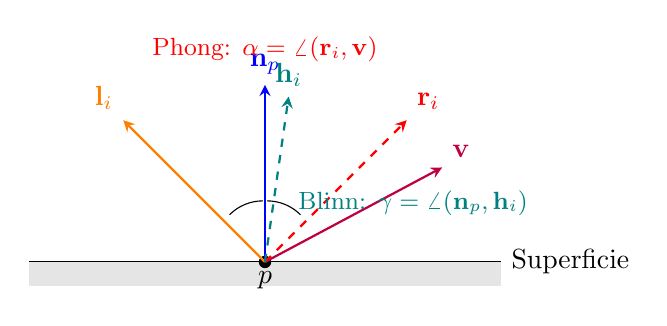
\begin{tikzpicture}[scale=1.5, >=stealth]
        % Superficie
        \draw[thick] (-2,0) -- (2,0) node[right] {Superficie};
        \fill[gray!20] (-2,0) rectangle (2,-0.2);
        \fill (0,0) circle (1.5pt) node[below] {$p$};
        
        % Vectores base
        \draw[->, thick, blue] (0,0) -- (0,1.5) node[above] {$\mathbf{n}_p$};
        \draw[->, thick, orange] (0,0) -- (-1.2, 1.2) node[above left] {$\mathbf{l}_i$};
        \draw[->, thick, purple] (0,0) -- (1.5, 0.8) node[above right] {$\mathbf{v}$};
        
        % Vector Reflejado (Phong)
        \draw[->, thick, red, dashed] (0,0) -- (1.2, 1.2) node[above right] {$\mathbf{r}_i$};
        \draw (-0.3, 0.4) arc (135:90:0.4);
        \draw (0.3, 0.4) arc (45:90:0.4);
        \node at (0, 1.8) [font=\small, color=red] {Phong: $\alpha = \angle(\mathbf{r}_i, \mathbf{v})$};
        
        % Vector Halfway (Blinn-Phong)
        % L = (-1.2, 1.2), V = (1.5, 0.8). Sum approx (0.3, 2). Normalized approx up.
        \draw[->, thick, teal, dashed] (0,0) -- (0.2, 1.4) node[above] {$\mathbf{h}_i$};
        \node at (0.2, 0.5) [font=\small, color=teal, right] {Blinn: $\gamma = \angle(\mathbf{n}_p, \mathbf{h}_i)$};
        
    \end{tikzpicture}
    \captionof{figure}{Esquema de vectores para Phong ($\mathbf{r}_i$) y Blinn-Phong ($\mathbf{h}_i$).}
    \end{center}
\end{ejercicio}

\begin{solucion}
    A continuación se detalla el procedimiento geométrico y la implementación en código GDScript para ambos modelos.
    
    \begin{enumerate}
        \item \textbf{Modelo de Sombreado de Phong ($f_{ph}$)}
        
        El modelo de Phong calcula el brillo especular basándose en el ángulo entre el vector de visión $\mathbf{v}$ y el vector de reflexión perfecta de la luz $\mathbf{r}_i$.
        
        \textit{Fórmulas requeridas:}
        \begin{itemize}
            \item Vector de reflexión: $\mathbf{r}_i = 2(\mathbf{n}_p \cdot \mathbf{l}_i)\mathbf{n}_p - \mathbf{l}_i$.
            \item Condición de luz incidente: $d_i = 1$ si $\mathbf{n}_p \cdot \mathbf{l}_i > 0$, de lo contrario $0$.
            \item Intensidad: $I = k_{ph} \cdot (\max(0, \mathbf{r}_i \cdot \mathbf{v}))^e$.
        \end{itemize}

        \textbf{Código GDScript:}
\begin{lstlisting}
func calcular_phong_especular(n: Vector3, v: Vector3, l: Vector3, e: float, k_ph: float) -> float:
    # 1. Calcular el producto punto entre la normal y la luz (Lambert)
    var n_dot_l : float = n.dot(l)
    
    # 2. Si la luz está detrás de la superficie, no hay especularidad
    if n_dot_l <= 0.0:
        return 0.0
        
    # 3. Calcular el vector reflejado r
    # Fórmula: r = 2 * (n . l) * n - l
    # En GDScript se puede usar reflect(), pero ojo: reflect devuelve 
    # el vector reflejado dada la dirección incidente y la normal. 
    # La fórmula manual es más explícita para teoría.
    var r : Vector3 = (2.0 * n_dot_l * n - l).normalized()
    
    # 4. Calcular el factor especular (r . v)^e
    var r_dot_v : float = max(0.0, r.dot(v))
    var specular : float = pow(r_dot_v, e)
    
    # 5. Devolver intensidad final ponderada por k_ph
    return k_ph * specular
\end{lstlisting}
        
        \vspace{0.5cm}
        
        \item \textbf{Modelo de Blinn-Phong ($f_{bp}$)}
        
        El modelo de Blinn-Phong optimiza el cálculo y suaviza el resultado utilizando el vector intermedio o \textit{halfway vector} $\mathbf{h}_i$, que es la bisectriz entre la luz $\mathbf{l}_i$ y la visión $\mathbf{v}$.
        
        \textit{Fórmulas requeridas:}
        \begin{itemize}
            \item Vector Halfway: $\mathbf{h}_i = \frac{\mathbf{l}_i + \mathbf{v}}{||\mathbf{l}_i + \mathbf{v}||}$.
            \item Intensidad: $I = k_{bp} \cdot (\mathbf{n}_p \cdot \mathbf{h}_i)^e$.
        \end{itemize}

        \textbf{Código GDScript:}
\begin{lstlisting}
func calcular_blinn_phong_especular(n: Vector3, v: Vector3, l: Vector3, e: float, k_bp: float) -> float:
    # 1. Calcular el producto punto N.L para descartar luz trasera
    var n_dot_l : float = n.dot(l)
    
    if n_dot_l <= 0.0:
        return 0.0
        
    # 2. Calcular el vector halfway (bisectriz) h
    # Es la suma de L y V, normalizada
    var h : Vector3 = (l + v).normalized()
    
    # 3. Calcular el producto punto entre la normal y el halfway vector
    var n_dot_h : float = max(0.0, n.dot(h))
    
    # 4. Elevar a la potencia (exponente de brillo)
    var specular : float = pow(n_dot_h, e)
    
    # 5. Devolver resultado ponderado
    return k_bp * specular
\end{lstlisting}
    \end{enumerate}
    
    \textit{Nota técnica:} En GDScript, la clase \texttt{Vector3} asume que los vectores ya están normalizados si el enunciado dice ''vectores unitarios''. Si no se garantiza, se debería llamar a \texttt{.normalized()} sobre los parámetros de entrada antes de operar.
\end{solucion}

\begin{ejercicio}
    \textbf{Cálculo de máximos de intensidad y visibilidad en una esfera.}

    Supongamos una esfera de radio unidad centrada en el origen.
    \begin{itemize}
        \item Se ilumina con una fuente de luz puntual en $\mathbf{p} = (0, 2, 0)$.
        \item El observador está situado en $\mathbf{o} = (2, 0, 0)$.
    \end{itemize}
    
    Determinar razonadamente el punto de la superficie donde el brillo será máximo y si dicho punto es visible para el observador para los siguientes casos:
    \begin{enumerate}
        \item Componente difusa (Lambertiana).
        \item Componente pseudo-especular de Phong.
        \item Componente pseudo-especular de Blinn-Phong.
    \end{enumerate}

    \begin{center}
    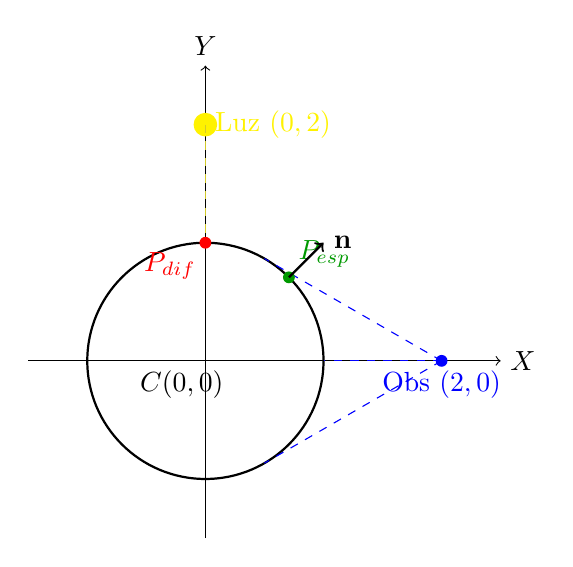
\begin{tikzpicture}[scale=1.5]
        % Ejes
        \draw[->] (-1.5,0) -- (2.5,0) node[right] {$X$};
        \draw[->] (0,-1.5) -- (0,2.5) node[above] {$Y$};
        
        % Esfera (círculo en 2D pues Z=0 para los puntos de interés)
        \draw[thick] (0,0) circle (1);
        \node at (-0.2,-0.2) {$C(0,0)$};
        
        % Luz
        \fill[yellow] (0,2) circle (0.1) node[right] {Luz $(0,2)$};
        \draw[dashed, yellow!80!black] (0,2) -- (0,1);
        
        % Observador
        \fill[blue] (2,0) circle (0.05) node[below] {Obs $(2,0)$};
        \draw[dashed, blue] (2,0) -- (1,0);
        \draw[dashed, blue] (2,0) -- (0.5, 0.866); % Tangente aprox
        \draw[dashed, blue] (2,0) -- (0.5, -0.866);
        
        % Punto Difuso
        \fill[red] (0,1) circle (0.05) node[below left] {$P_{dif}$};
        
        % Punto Especular
        \fill[green!60!black] (0.707,0.707) circle (0.05) node[above right] {$P_{esp}$};
        
        % Vector Normal en P_esp
        \draw[->, thick] (0.707,0.707) -- (1.0, 1.0) node[right] {$\mathbf{n}$};
        
    \end{tikzpicture}
    \captionof{figure}{Diagrama de la escena en el plano $XY$ ($z=0$).}
    \end{center}
\end{ejercicio}

\begin{solucion}
    Analizaremos cada caso paso a paso. Dado que tanto la luz como el observador están en el plano $XY$ ($z=0$) y la esfera está centrada en el origen, los puntos de máximo brillo estarán necesariamente en el círculo máximo del plano $XY$.
    
    Datos geométricos generales para un punto $P(x,y,z)$ en la superficie de la esfera unitaria:
    \begin{itemize}
        \item Radio $R=1$, Centro $C=(0,0,0)$.
        \item La normal en la superficie es $\mathbf{n}_p = P - C = (x,y,z)$.
        \item Vector hacia la luz: $\mathbf{l} = \text{normalizar}(\mathbf{p} - P)$.
        \item Vector hacia el observador: $\mathbf{v} = \text{normalizar}(\mathbf{o} - P)$.
    \end{itemize}

    \textbf{Condición de Visibilidad:} 
    Un punto $P$ es visible si el ángulo entre la normal $\mathbf{n}_p$ y el vector de visión $\mathbf{v}$ es menor de 90 grados, es decir, $\mathbf{n}_p \cdot \mathbf{v} > 0$.
    
    Analicemos el horizonte de visibilidad para el observador en $(2,0,0)$:
    $$ \mathbf{v}_{aprox} \approx (2,0,0) - (x,y,z) = (2-x, -y, -z) $$
    $$ \mathbf{n}_p \cdot \mathbf{v}_{aprox} \propto (x,y,z) \cdot (2-x, -y, -z) = 2x - (x^2+y^2+z^2) = 2x - 1 $$
    La condición $\mathbf{n}_p \cdot \mathbf{v} > 0 \implies 2x - 1 > 0 \implies x > 0.5$.
    \textit{Cualquier punto con coordenada $x \le 0.5$ está oculto por el horizonte de la esfera.}

    \begin{enumerate}
        \item \textbf{Componente Difusa (Lambertiana)}
        
        La intensidad difusa es proporcional a $\mathbf{n}_p \cdot \mathbf{l}$. El brillo es máximo cuando la normal apunta directamente a la luz ($\mathbf{n}_p \parallel \mathbf{l}$).
        
        \begin{itemize}
            \item Dirección desde el centro a la luz: $(0,2,0) - (0,0,0) = (0,2,0)$.
            \item El punto de la superficie en esa dirección es $P_{dif} = (0, 1, 0)$.
            \item \textbf{Visibilidad:} La coordenada $x$ de $P_{dif}$ es $0$.
            \item Como $0 \le 0.5$, el punto \textbf{NO es visible}. Está en la parte superior de la esfera, pero el observador, situado a la derecha, solo ve hasta $x > 0.5$.
        \end{itemize}

        \item \textbf{Componente Pseudo-especular (Phong)}
        
        La intensidad es proporcional a $(\mathbf{r} \cdot \mathbf{v})^e$, donde $\mathbf{r}$ es el reflejo de la luz sobre la normal. El máximo ocurre cuando $\mathbf{r} = \mathbf{v}$ (reflexión perfecta). Esto implica que la normal $\mathbf{n}_p$ debe ser la bisectriz del ángulo formado por el vector luz $\mathbf{l}$ y el vector visión $\mathbf{v}$.
        
        Debido a la simetría del problema (Luz en eje Y, Observador en eje X, distancias iguales al origen), el punto debe estar en la bisectriz del primer cuadrante ($x=y$).
        
        \begin{itemize}
            \item Punto en la esfera a 45 grados: $P_{esp} = (\cos(45^\circ), \sin(45^\circ), 0) = \left(\frac{\sqrt{2}}{2}, \frac{\sqrt{2}}{2}, 0\right) \approx (0.707, 0.707, 0)$.
            \item Comprobación geométrica: La normal en este punto apunta a $(1,1)$. La luz está en $(0,2)$ y el ojo en $(2,0)$. El vector normal divide simétricamente el ángulo entre la luz y el ojo.
            \item \textbf{Visibilidad:} La coordenada $x$ de $P_{esp}$ es $0.707$.
            \item Como $0.707 > 0.5$, el punto \textbf{SÍ es visible}. El brillo especular aparecerá en el ''hombro'' de la esfera mirando hacia el observador.
        \end{itemize}

        \item \textbf{Modelo de Blinn-Phong}
        
        La intensidad es proporcional a $(\mathbf{n}_p \cdot \mathbf{h})^e$, donde $\mathbf{h}$ (halfway vector) es la bisectriz entre $\mathbf{l}$ y $\mathbf{v}$. El máximo ocurre cuando la normal $\mathbf{n}_p$ coincide con $\mathbf{h}$.
        
        \begin{itemize}
            \item Geométricamente, la condición ''la normal coincide con la bisectriz de L y V'' es idéntica a la condición de reflexión perfecta del modelo de Phong descrita arriba.
            \item Por tanto, el punto de máximo brillo es el mismo: $P_{bp} = \left(\frac{\sqrt{2}}{2}, \frac{\sqrt{2}}{2}, 0\right)$.
            \item \textbf{Visibilidad:} Al ser el mismo punto, \textbf{SÍ es visible}.
        \end{itemize}
    \end{enumerate}
\end{solucion}

\begin{ejercicio}
    \textbf{Evaluación de la BRDF de Microfacetas (GGX).}

    Escribe el código en GDScript de una función para calcular la reflectividad debida a la BRDF de microfacetas GGX, evaluando la expresión de $f_{ggx}$ (Ecuación 10).
    
    La función recibirá los siguientes parámetros:
    \begin{itemize}
        \item Vectores unitarios: Dirección de iluminación ($\mathbf{w}_i$), dirección de visión ($\mathbf{w}_o$), tangente X ($\mathbf{t}_x$), tangente Y ($\mathbf{t}_y$) y normal de la macrosuperficie ($\mathbf{n}_x$).
        \item Valores de rugosidad: $\alpha_x$ y $\alpha_y$ (tipo float).
    \end{itemize}
    
    La función debe devolver un valor de tipo \texttt{float}.

    \vspace{0.5cm}
    
    % Diagrama de Microfacetas GGX
    \begin{center}
    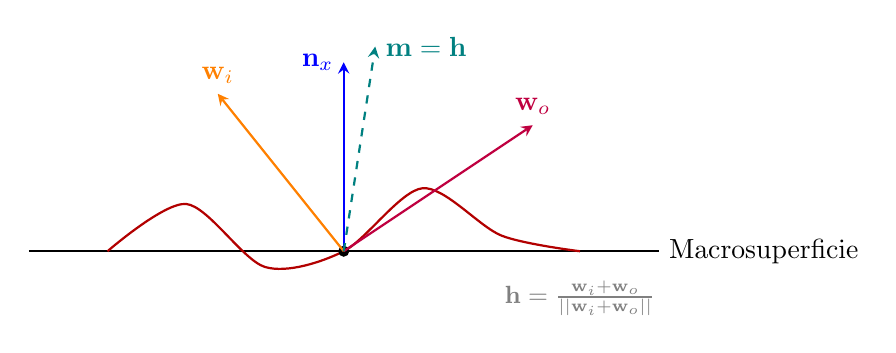
\begin{tikzpicture}[scale=2, >=stealth]
        % Macrosuperficie
        \draw[thick] (-2,0) -- (2,0) node[right] {Macrosuperficie};
        
        % Microfaceta (curva representativa)
        \draw[thick, red!70!black, smooth] plot coordinates {(-1.5,0) (-1, 0.3) (-0.5, -0.1) (0, 0) (0.5, 0.4) (1, 0.1) (1.5, 0)};
        
        % Punto de evaluación
        \fill (0,0) circle (1pt);
        
        % Vectores principales
        \draw[->, thick, blue] (0,0) -- (0,1.2) node[left] {$\mathbf{n}_x$};
        \draw[->, thick, orange] (0,0) -- (-0.8, 1.0) node[above] {$\mathbf{w}_i$};
        \draw[->, thick, purple] (0,0) -- (1.2, 0.8) node[above] {$\mathbf{w}_o$};
        
        % Vector Halfway (Normal de la microfaceta activa)
        \draw[->, thick, teal, dashed] (0,0) -- (0.2, 1.3) node[right] {$\mathbf{m} = \mathbf{h}$};
        
        % Anotación
        \node at (1.5, -0.3) [font=\small, color=gray] {$\mathbf{h} = \frac{\mathbf{w}_i + \mathbf{w}_o}{||\mathbf{w}_i + \mathbf{w}_o||}$};
    \end{tikzpicture}
    \captionof{figure}{Geometría de microfacetas: El vector $\mathbf{h}$ actúa como la normal de la microfaceta ($\mathbf{m}$) que refleja $\mathbf{w}_i$ hacia $\mathbf{w}_o$.}
    \end{center}
\end{ejercicio}

\begin{solucion}
    Para implementar la BRDF GGX completa, debemos desglosar la Ecuación 10 en sus tres componentes principales: la Distribución de Normales ($D$), el Enmascaramiento-Sombreado ($G$) y el término de Fresnel ($F$).
    
    \begin{enumerate}
        \item \textbf{Cálculo del Vector Halfway ($\mathbf{h}$):}
        Es la bisectriz entre el vector de luz y el de visión. Representa la orientación que debe tener una microfaceta para reflejar la luz perfectamente hacia el observador.
        $$ \mathbf{h} = \frac{\mathbf{w}_i + \mathbf{w}_o}{||\mathbf{w}_i + \mathbf{w}_o||} $$
        
        \item \textbf{Distribución de Normales Anisotrópica ($D$):}
        Evaluamos la probabilidad de que una microfaceta esté alineada con $\mathbf{h}$. Usamos la fórmula GGX anisotrópica (Ecuación de transparencia 75):
        $$ D(\mathbf{h}) = \frac{1}{\pi \alpha_x \alpha_y \left( (\frac{\mathbf{h} \cdot \mathbf{t}_x}{\alpha_x})^2 + (\frac{\mathbf{h} \cdot \mathbf{t}_y}{\alpha_y})^2 + (\mathbf{h} \cdot \mathbf{n}_x)^2 \right)^2} $$
        
        \item \textbf{Enmascaramiento y Sombreado ($G_2$):}
        Usamos la aproximación \textit{Height Correlated Masking and Shadowing} (Ecuación de transparencia 77). Se define mediante una función auxiliar $\Lambda(w)$:
        $$ \Lambda(\mathbf{w}) = \frac{1}{2} \left( -1 + \sqrt{1 + \frac{\alpha_x^2 x^2 + \alpha_y^2 y^2}{z^2}} \right) $$
        Donde $x, y, z$ son las proyecciones del vector $\mathbf{w}$ sobre $\mathbf{t}_x, \mathbf{t}_y, \mathbf{n}_x$.
        $$ G_2 = \frac{1}{1 + \Lambda(\mathbf{w}_i) + \Lambda(\mathbf{w}_o)} $$
        
        \item \textbf{Término de Fresnel ($F$):}
        Usamos la aproximación de Schlick (Ecuación de transparencia 78). Aunque el enunciado no proporciona el índice de refracción ($f_0$), es necesario para la ecuación. Asumiremos un valor estándar de $0.04$ (dieléctrico común) para completar el cálculo.
        $$ F \approx f_0 + (1 - f_0)(1 - (\mathbf{w}_i \cdot \mathbf{h}))^5 $$
        
        \item \textbf{Combinación Final ($f_{ggx}$):}
        $$ f_{ggx} = \frac{F \cdot D \cdot G_2}{4 (\mathbf{w}_i \cdot \mathbf{n}_x) (\mathbf{w}_o \cdot \mathbf{n}_x)} $$
    \end{enumerate}

    \textbf{Implementación en GDScript:}

\begin{lstlisting}
func calcular_brdf_ggx(wi: Vector3, wo: Vector3, tx: Vector3, ty: Vector3, nx: Vector3, ax: float, ay: float) -> float:
    # 1. Calcular el vector Halfway (h)
    var h: Vector3 = (wi + wo).normalized()
    
    # Pre-cálculo de productos punto necesarios
    var n_dot_wi = max(0.0001, nx.dot(wi)) # Evitar división por cero
    var n_dot_wo = max(0.0001, nx.dot(wo))
    var n_dot_h  = max(0.0, nx.dot(h))
    var h_dot_wi = max(0.0, h.dot(wi))
    
    # Proyecciones para anisotropía
    var h_dot_tx = h.dot(tx)
    var h_dot_ty = h.dot(ty)
    
    # 2. Calcular Distribución D (GGX Anisotrópica)
    var term_x = pow(h_dot_tx / ax, 2)
    var term_y = pow(h_dot_ty / ay, 2)
    var term_z = pow(n_dot_h, 2)
    
    var denom_d = PI * ax * ay * pow(term_x + term_y + term_z, 2)
    var D = 1.0 / max(0.0001, denom_d)
    
    # 3. Calcular Geometría G2 (Height Correlated)
    # Función Lambda auxiliar inline para wi
    var wi_x = wi.dot(tx) * ax
    var wi_y = wi.dot(ty) * ay
    var wi_z = n_dot_wi
    var lambda_wi = 0.5 * (-1.0 + sqrt(1.0 + (pow(wi_x, 2) + pow(wi_y, 2)) / pow(wi_z, 2)))
    
    # Función Lambda auxiliar inline para wo
    var wo_x = wo.dot(tx) * ax
    var wo_y = wo.dot(ty) * ay
    var wo_z = n_dot_wo
    var lambda_wo = 0.5 * (-1.0 + sqrt(1.0 + (pow(wo_x, 2) + pow(wo_y, 2)) / pow(wo_z, 2)))
                    
    var G2 = 1.0 / (1.0 + lambda_wi + lambda_wo)
    
    # 4. Calcular Fresnel F (Aproximación de Schlick)
    var f0 = 0.04 # Valor asumido para dieléctricos si no se provee
    var F = f0 + (1.0 - f0) * pow(1.0 - h_dot_wi, 5)
    
    # 5. Resultado final combinado
    var numerador = F * D * G2
    var denominador = 4.0 * n_dot_wi * n_dot_wo
    
    return numerador / max(0.0001, denominador)
\end{lstlisting}
\end{solucion}

\section{Sesión 8}

\begin{ejercicio}
%\textbf{Problema 8.1: Coordenadas de textura.}
Supongamos que se desea crear una malla indexada para un cubo, de forma que deseamos aplicar una textura que incluya las caras de un dado. Para ello disponemos de una imagen de textura que tiene una relación de aspecto 4:3.
\begin{center}
% Dibujo de la cruz de un dado (desplegable de cubo) usando TikZ
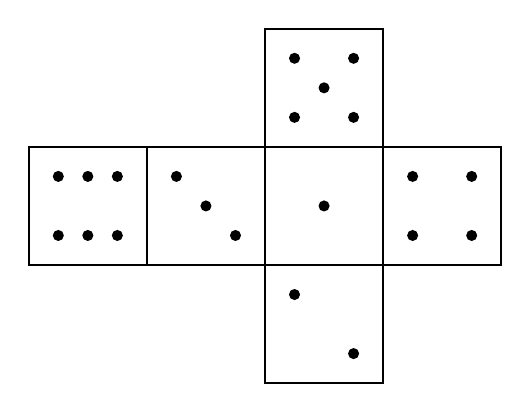
\begin{tikzpicture}[scale=1.5, dot/.style={circle, fill=black, minimum size=4pt, inner sep=0pt}]
    % Definición de las caras (cuadrados)
    % Centro (1), Arriba (5), Abajo (2), Izquierda (3), Derecha (4), Extrema Izquierda (6)
    \foreach \x/\y in {0/0, 0/1, 0/-1, -1/0, 1/0, -2/0} {
        \draw[thick] (\x-0.5,\y-0.5) rectangle (\x+0.5,\y+0.5);
    }

    % Cara Central (1 punto)
    \node[dot] at (0,0) {};

    % Cara Superior (5 puntos)
    \node[dot] at (0,1) {};
    \node[dot] at (-0.25,1.25) {};
    \node[dot] at (0.25,1.25) {};
    \node[dot] at (-0.25,0.75) {};
    \node[dot] at (0.25,0.75) {};

    % Cara Inferior (2 puntos - diagonal invertida según imagen)
    \node[dot] at (-0.25,-0.75) {};
    \node[dot] at (0.25,-1.25) {};

    % Cara Derecha (4 puntos)
    \node[dot] at (0.75,0.25) {};
    \node[dot] at (1.25,0.25) {};
    \node[dot] at (0.75,-0.25) {};
    \node[dot] at (1.25,-0.25) {};

    % Cara Izquierda (3 puntos - diagonal)
    \node[dot] at (-1.25,0.25) {};
    \node[dot] at (-1,0) {};
    \node[dot] at (-0.75,-0.25) {};

    % Cara Extrema Izquierda (6 puntos)
    \node[dot] at (-2.25,0.25) {};
    \node[dot] at (-2,0.25) {};
    \node[dot] at (-1.75,0.25) {};
    \node[dot] at (-2.25,-0.25) {};
    \node[dot] at (-2,-0.25) {};
    \node[dot] at (-1.75,-0.25) {};

\end{tikzpicture}
\end{center}
\begin{enumerate}
    \item Describe razonadamente cuántos vértices (como mínimo) tendrá el modelo.
    \item Escribe la tabla de coordenadas de vértices, la tabla de coordenadas de textura y la tabla de triángulos. Ten en cuenta que el cubo tiene lado unidad y su centro está en $(0.5, 0.5, 0.5)$.
    \item Dibuja un esquema de la textura en la cual cada vértice del modelo aparezca etiquetado con su número de vértice más sus coordenadas de textura.
\end{enumerate}
\end{ejercicio}

\begin{solucion}
\begin{enumerate} 

La resolución del ejercicio es la siguiente:
\item Número de Vértices del Modelo

Aunque un cubo geométrico estándar tiene 8 vértices espaciales (esquinas), en informática gráfica, un vértice en una malla indexada se define como una tupla única de atributos: $(x, y, z, u, v, \dots)$. Si un mismo punto geométrico (esquina del cubo) necesita tener dos coordenadas de textura distintas (por ejemplo, en una costura donde la textura se corta), el vértice debe duplicarse.

Observando la distribución de la textura en cruz proporcionada en las diapositivas, la imagen tiene un aspect ratio 4:3, lo que implica una rejilla de $4 \times 3$ caras. La disposición es:
\begin{itemize}
    \item Fila superior: Cara 5.
    \item Fila media: Caras 6, 3, 1, 4.
    \item Fila inferior: Cara 2.
\end{itemize}

Para calcular el número mínimo de vértices, analizamos la conectividad en el espacio UV:
\begin{itemize}
    \item Si tratamos cada cara como un cuadrado independiente, tendríamos $6 \times 4 = 24$ vértices.
    \item Restamos los vértices que se comparten en las aristas continuas en la textura (donde no hay corte UV). Las conexiones visuales son: 6-3, 3-1, 1-4, 5-1 y 1-2.
    \item Hay 5 aristas compartidas. Cada arista fusiona 2 pares de vértices.
    \item Total vértices = $24 - (5 \text{ aristas} \times 2 \text{ vértices}) = 14$.
\end{itemize}

Por tanto, el modelo necesita \textbf{14 vértices} únicos.
\vspace{1cm}
\item  Tablas de Definición del Modelo

Asumimos el sistema de referencia donde la cara 1 es el Frontal ($z=1$), la cara 5 es Arriba ($y=1$), la cara 2 es Abajo ($y=0$), la cara 3 es Izquierda ($x=0$), la cara 4 es Derecha ($x=1$) y la cara 6 es Atrás ($z=0$).
El cubo va de $(0,0,0)$ a $(1,1,1)$.

Dividimos el dominio de textura $u \in [0,1], v \in [0,1]$ según la rejilla 4x3\footnote{Es en base al enunciado.}:
\begin{itemize}
    \item Paso en $u$: $1/4 = 0.25$. Columnas: $0, 0.25, 0.5, 0.75, 1.0$.
    \item Paso en $v$: $1/3 \approx 0.333$. Filas: $0, 0.33, 0.66, 1.0$.
\end{itemize}

\textit{Nota:} Las divisiones que se hacen de u y v corresponden a cada vértice, de manera que tan solo tenemos que imaginar que la textura es como una tabla, si vemos en la cara 5 (arriba) esta entre u=0.5 a u=0.75 y v=0.66 a v=1.0. En la tabla se hace referencia a top-esquina, lo que se conoce como top-left en inglés, por ende, debemos debemos de tener en cuenta que la coordenada v=1.0 es la parte superior de la textura y v=0.0 es la parte inferior. Se le debe de atribuir u=0.5 y v=1.0 a la esquina superior izquierda de la cara 5 (arriba).


\vspace{1cm}
\underline{Tabla de Vértices (Geometría + Textura)} \\\\
Ordenamos los vértices recorriendo la textura de arriba a abajo y de izquierda a derecha.

\begin{center}
\begin{tabular}{|c|c|c|c|}
\hline
\textbf{Índice ($i$)} & \textbf{Posición $(x, y, z)$} & \textbf{Coord. Textura $(u, v)$} & \textbf{Descripción (UV)} \\ \hline
0 & $(0, 1, 0)$ & $(0.50, 1.00)$ & Top-Esq Cara 5 \\ \hline
1 & $(1, 1, 0)$ & $(0.75, 1.00)$ & Top-Der Cara 5 \\ \hline
2 & $(1, 1, 0)$ & $(0.00, 0.66)$ & Top-Esq Cara 6 \\ \hline
3 & $(0, 1, 0)$ & $(0.25, 0.66)$ & Top-Der 6 / Top-Esq 3 \\ \hline
4 & $(0, 1, 1)$ & $(0.50, 0.66)$ & Top-Der 3 / Top-Esq 1 / Bot-Esq 5 \\ \hline
5 & $(1, 1, 1)$ & $(0.75, 0.66)$ & Top-Der 1 / Top-Esq 4 / Bot-Der 5 \\ \hline
6 & $(1, 1, 0)$ & $(1.00, 0.66)$ & Top-Der 4 \\ \hline
7 & $(1, 0, 0)$ & $(0.00, 0.33)$ & Bot-Esq Cara 6 \\ \hline
8 & $(0, 0, 0)$ & $(0.25, 0.33)$ & Bot-Der 6 / Bot-Esq 3 \\ \hline
9 & $(0, 0, 1)$ & $(0.50, 0.33)$ & Bot-Der 3 / Bot-Esq 1 / Top-Esq 2 \\ \hline
10 & $(1, 0, 1)$ & $(0.75, 0.33)$ & Bot-Der 1 / Bot-Esq 4 / Top-Der 2 \\ \hline
11 & $(1, 0, 0)$ & $(1.00, 0.33)$ & Bot-Der 4 \\ \hline
12 & $(0, 0, 0)$ & $(0.50, 0.00)$ & Bot-Esq Cara 2 \\ \hline
13 & $(1, 0, 0)$ & $(0.75, 0.00)$ & Bot-Der Cara 2 \\ \hline
\end{tabular}
\end{center}
\vspace{1cm}
\underline{Tabla de Triángulos} \\\\
Definimos dos triángulos por cara (sentido antihorario visto desde fuera).

\begin{center}
\begin{tabular}{|c|c|c|}
\hline
\textbf{Cara (Dado)} & \textbf{Triángulo 1 $(v_a, v_b, v_c)$} & \textbf{Triángulo 2 $(v_a, v_c, v_d)$} \\ \hline
5 (Arriba) & $(0, 1, 4)$ & $(1, 5, 4)$ \\ \hline
6 (Atrás) & $(2, 3, 7)$ & $(3, 8, 7)$ \\ \hline
3 (Izq) & $(3, 4, 8)$ & $(4, 9, 8)$ \\ \hline
1 (Frente) & $(4, 5, 9)$ & $(5, 10, 9)$ \\ \hline
4 (Der) & $(5, 6, 10)$ & $(6, 11, 10)$ \\ \hline
2 (Abajo) & $(9, 10, 12)$ & $(10, 13, 12)$ \\ \hline
\end{tabular}
\end{center}

\textit{Nota:} Usamos orden horario.

\vspace{1cm}
\item Esquema de la Textura

A continuación se muestra el espacio de coordenadas de textura $(u,v)$ con los vértices etiquetados según la tabla anterior.

\begin{center}
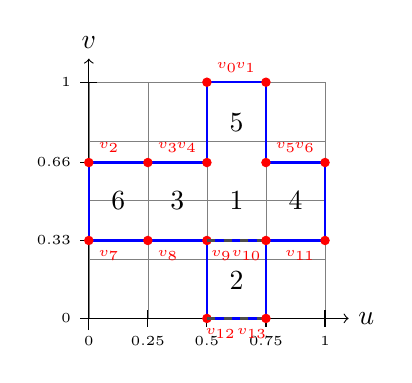
\begin{tikzpicture}[scale=3]
    % Draw grid
    \draw[step=0.25cm,gray,very thin] (0,0) grid (1,1);
    
    % Draw axes
    \draw[->] (0,0) -- (1.1,0) node[right] {$u$};
    \draw[->] (0,-0.05) -- (0,1.1) node[above] {$v$};
    
    % Ticks
    \foreach \x in {0, 0.25, 0.5, 0.75, 1} \draw (\x,1pt) -- (\x,-1pt) node[anchor=north, font=\tiny] {\x};
    \foreach \y/\yl in {0/0, 0.33/0.33, 0.66/0.66, 1/1} \draw (1pt,\y) -- (-1pt,\y) node[anchor=east, font=\tiny] {\yl};

    % Draw Texture Map Outline (The Cross)
    \draw[thick, blue] (0, 0.33) -- (1, 0.33) -- (1, 0.66) -- (0.75, 0.66) -- (0.75, 1) -- (0.5, 1) -- (0.5, 0.66) -- (0, 0.66) -- cycle;
    \draw[thick, blue] (0.5, 0.33) -- (0.5, 0) -- (0.75, 0) -- (0.75, 0.33);
    
    % Fill Faces labels
    \node at (0.125, 0.5) {6};
    \node at (0.375, 0.5) {3};
    \node at (0.625, 0.5) {1};
    \node at (0.875, 0.5) {4};
    \node at (0.625, 0.83) {5};
    \node at (0.625, 0.16) {2};

    % Plot Vertices
    % Row v=1
    \filldraw [red] (0.5, 1) circle (0.5pt) node[above right, font=\tiny] {$v_0$};
    \filldraw [red] (0.75, 1) circle (0.5pt) node[above left, font=\tiny] {$v_1$};
    
    % Row v=0.66
    \filldraw [red] (0, 0.66) circle (0.5pt) node[above right, font=\tiny] {$v_2$};
    \filldraw [red] (0.25, 0.66) circle (0.5pt) node[above right, font=\tiny] {$v_3$};
    \filldraw [red] (0.5, 0.66) circle (0.5pt) node[above left, font=\tiny] {$v_4$};
    \filldraw [red] (0.75, 0.66) circle (0.5pt) node[above right, font=\tiny] {$v_5$};
    \filldraw [red] (1, 0.66) circle (0.5pt) node[above left, font=\tiny] {$v_6$};

    % Row v=0.33
    \filldraw [red] (0, 0.33) circle (0.5pt) node[below right, font=\tiny] {$v_7$};
    \filldraw [red] (0.25, 0.33) circle (0.5pt) node[below right, font=\tiny] {$v_8$};
    \filldraw [red] (0.5, 0.33) circle (0.5pt) node[below right, font=\tiny, xshift=-2pt] {$v_9$};
    % Separation between v9 and v10
    \draw[dashed, gray!60!black, thick] (0.5,0.33) -- (0.75,0.33);
    \filldraw [red] (0.75, 0.33) circle (0.5pt) node[below left, font=\tiny, xshift=2pt] {$v_{10}$};
    \filldraw [red] (1, 0.33) circle (0.5pt) node[below left, font=\tiny] {$v_{11}$};

    % Row v=0
    \filldraw [red] (0.5, 0) circle (0.5pt) node[below right, font=\tiny, xshift=-4pt] {$v_{12}$};
    % Separation between v12 and v13
    \draw[dashed, gray!60!black, thick] (0.5,0) -- (0.75,0);
    \filldraw [red] (0.75, 0) circle (0.5pt) node[below left, font=\tiny, xshift=4pt] {$v_{13}$};

\end{tikzpicture}
\end{center}
\end{enumerate}

El código GDScript para definir las tablas de vértices, coordenadas de textura y triángulos es el siguiente:
\begin{lstlisting}[language=gdscript]
# Definición de los vértices: posición y coordenadas de textura
var vertices = [
    Vector3(0, 1, 0),   # v0
    Vector3(1, 1, 0),   # v1
    Vector3(1, 1, 0),   # v2
    Vector3(0, 1, 0),   # v3
    Vector3(0, 1, 1),   # v4
    Vector3(1, 1, 1),   # v5
    Vector3(1, 1, 0),   # v6
    Vector3(1, 0, 0),   # v7
    Vector3(0, 0, 0),   # v8
    Vector3(0, 0, 1),   # v9
    Vector3(1, 0, 1),   # v10
    Vector3(1, 0, 0),   # v11
    Vector3(0, 0, 0),   # v12
    Vector3(1, 0, 0),   # v13
]

var uvs = [
    Vector2(0.50, 1.00),   # v0
    Vector2(0.75, 1.00),   # v1
    Vector2(0.00, 0.66),   # v2
    Vector2(0.25, 0.66),   # v3
    Vector2(0.50, 0.66),   # v4
    Vector2(0.75, 0.66),   # v5
    Vector2(1.00, 0.66),   # v6
    Vector2(0.00, 0.33),   # v7
    Vector2(0.25, 0.33),   # v8
    Vector2(0.50, 0.33),   # v9
    Vector2(0.75, 0.33),   # v10
    Vector2(1.00, 0.33),   # v11
    Vector2(0.50, 0.00),   # v12
    Vector2(0.75, 0.00),   # v13
]

# Definición de los triángulos (índices de vértices) en orden horario (sentido antihorario visto desde fuera)
var triangles = [
    # Cara 5 (Arriba)
    0, 1, 4,
    1, 5, 4,
    # Cara 6 (Atrás)
    2, 3, 7,
    3, 8, 7,
    # Cara 3 (Izquierda)
    3, 4, 8,
    4, 9, 8,
    # Cara 1 (Frente)
    4, 5, 9,
    5, 10, 9,
    # Cara 4 (Derecha)
    5, 6, 10,
    6, 11, 10,
    # Cara 2 (Abajo)
    9, 10, 12,
    10, 13, 12,
]
\end{lstlisting}
\end{solucion}

\begin{ejercicio}
%\textbf{Problema 8.2:}
Considera de nuevo el cubo y la textura del problema anterior (un cubo de lado unidad con centro en $(0.5, 0.5, 0.5)$ y una textura de imagen con relación de aspecto 4:3 que despliega las caras de un dado). Supón que ahora queremos visualizar el cubo iluminado, para lo cual debemos asignar normales a los vértices.

Responde a estas cuestiones:
\begin{enumerate}
    \item Describe razonadamente si sería posible usar la misma tabla de vértices y la misma tabla de coordenadas de textura que en el problema anterior (donde se buscaba el número mínimo de vértices), o si es necesario usar tablas distintas.
    \item Si has respondido que no es posible usar las mismas tablas, escribe la nueva tabla de vértices, la nueva tabla de coordenadas de textura y la tabla de normales.
\end{enumerate}
\end{ejercicio}

\begin{solucion} La resolución del ejercicio es la siguiente:

\textbf{1. Análisis de la reutilización de la tabla de vértices}

Para responder a esta cuestión, debemos entender qué define un \textit{vértice} en el contexto del cauce gráfico (pipeline) cuando aplicamos iluminación.

En el problema anterior (8.1), buscábamos minimizar el espacio geométrico. Un cubo tiene geométricamente 8 esquinas. Si solo nos importara la posición $(x, y, z)$, podríamos definir solo 8 vértices y reutilizarlos mediante índices.

Sin embargo, para la iluminación (sombreado), necesitamos asociar un \textbf{vector normal} ($\vec{n}$) a cada vértice. El vector normal indica hacia dónde ''mira'' la superficie en ese punto para calcular cómo rebota la luz.

\begin{itemize}
    \item \textbf{El problema de la continuidad:} En una esfera suave, la normal en un vértice es el promedio de las caras adyacentes, permitiendo un sombreado suave (Gouraud).
    \item \textbf{El caso del cubo (aristas vivas):} Un cubo tiene aristas afiladas (no suaves). Consideremos una esquina del cubo, por ejemplo, la superior-derecha-frontal $(1, 1, 1)$.
    \begin{itemize}
        \item Para la cara \textbf{Frontal}, la normal debe apuntar hacia adelante: $\vec{n} = (0, 0, 1)$.
        \item Para la cara \textbf{Superior}, la normal debe apuntar hacia arriba: $\vec{n} = (0, 1, 0)$.
        \item Para la cara \textbf{Derecha}, la normal debe apuntar a la derecha: $\vec{n} = (1, 0, 0)$.
    \end{itemize}
\end{itemize}

Como un vértice en la memoria de la GPU es una estructura de datos única que contiene $\{Posici\acute{o}n, Normal, UV\}$, no podemos tener un solo vértice con tres normales distintas simultáneamente.

\vspace{0.3cm}
\begin{center}
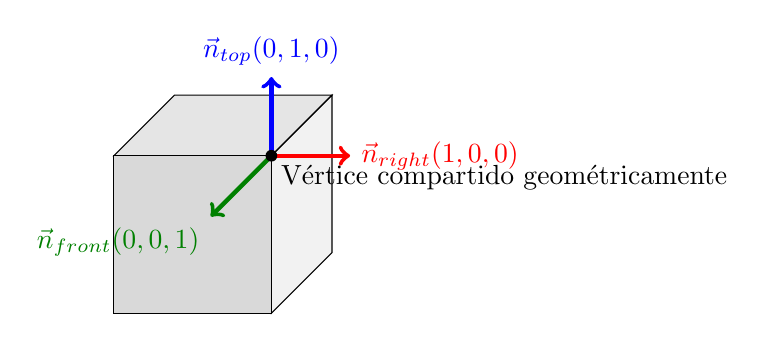
\begin{tikzpicture}[scale=2]
    % Coordenadas del cubo
    \coordinate (O) at (0,0,0);
    \coordinate (A) at (1,0,0);
    \coordinate (B) at (1,1,0);
    \coordinate (C) at (0,1,0);
    \coordinate (D) at (0,0,1);
    \coordinate (E) at (1,0,1);
    \coordinate (F) at (1,1,1);
    \coordinate (G) at (0,1,1);

    % Caras
    \draw[fill=gray!20] (F) -- (G) -- (C) -- (B) -- cycle; % Top
    \draw[fill=gray!10] (F) -- (E) -- (A) -- (B) -- cycle; % Right
    \draw[fill=gray!30] (F) -- (G) -- (D) -- (E) -- cycle; % Front

    % Aristas
    \draw (F) -- (G);
    \draw (F) -- (E);
    \draw (F) -- (B);

    % Vector Normales en el vertice F
    \draw[->, ultra thick, blue] (F) -- +(0, 0.5, 0) node[above] {$\vec{n}_{top} (0,1,0)$};
    \draw[->, ultra thick, red] (F) -- +(0.5, 0, 0) node[right] {$\vec{n}_{right} (1,0,0)$};
    \draw[->, ultra thick, green!50!black] (F) -- +(0, 0, 1) node[below left] {$\vec{n}_{front} (0,0,1)$};

    \node at (F) [circle, fill, inner sep=1.5pt] {};
    \node[below right] at (F) {Vértice compartido geométricamente};
\end{tikzpicture}
\end{center}
\vspace{0.3cm}

\textbf{Conclusión:} \textbf{No es posible} usar la misma tabla reducida de 8 vértices. Es necesario duplicar los vértices en las costuras de las aristas. Necesitaremos vértices independientes para cada cara del cubo.
\\
Total de vértices necesarios: $6 \text{ caras} \times 4 \text{ vértices/cara} = \textbf{24 vértices}$.

\vspace{0.5cm}

\textbf{2. Definición de las nuevas tablas}

Para construir las tablas, asumiremos la disposición de textura ''en cruz'' típica para una relación de aspecto 4:3, tal como sugiere el enunciado del Problema 8.1.

\textbf{Esquema de la Textura (Relación 4:3):}
Dividimos la textura en una cuadrícula de $4 \times 3$.
\begin{itemize}
    \item Ancho de celda ($u$): $1/4 = 0.25$
    \item Alto de celda ($v$): $1/3 \approx 0.333$
\end{itemize}

\begin{center}
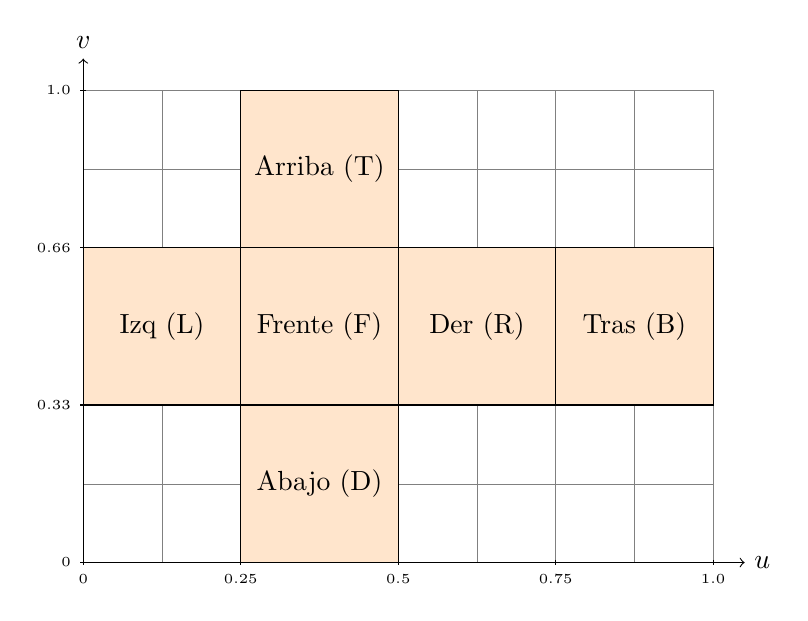
\begin{tikzpicture}[x=2cm, y=2cm]
    \draw[step=1cm, gray, very thin] (0,0) grid (4,3);
    
    % Dibujar la cruz del dado
    \draw[fill=orange!20] (0,1) rectangle (1,2) node[pos=.5] {Izq (L)};
    \draw[fill=orange!20] (1,1) rectangle (2,2) node[pos=.5] {Frente (F)};
    \draw[fill=orange!20] (2,1) rectangle (3,2) node[pos=.5] {Der (R)};
    \draw[fill=orange!20] (3,1) rectangle (4,2) node[pos=.5] {Tras (B)};
    \draw[fill=orange!20] (1,2) rectangle (2,3) node[pos=.5] {Arriba (T)};
    \draw[fill=orange!20] (1,0) rectangle (2,1) node[pos=.5] {Abajo (D)};
    
    % Ejes UV
    \draw[->] (0,0) -- (4.2,0) node[right] {$u$};
    \draw[->] (0,0) -- (0,3.2) node[above] {$v$};
    
    % Etiquetas coordenadas
    \foreach \x/\label in {0/0, 1/0.25, 2/0.5, 3/0.75, 4/1.0}
        \draw (\x, 1pt) -- (\x, -1pt) node[below, font=\tiny] {\label};
    \foreach \y/\label in {0/0, 1/0.33, 2/0.66, 3/1.0}
        \draw (1pt, \y) -- (-1pt, \y) node[left, font=\tiny] {\label};
\end{tikzpicture}
\end{center}

A continuación, definimos las tablas. Dado que el cubo tiene lado 1 y centro en $(0.5, 0.5, 0.5)$, las coordenadas van de $0.0$ a $1.0$ en los ejes X, Y, Z.

\textbf{Nota de notación:}
\begin{itemize}
    \item \textbf{Posición:} $(x, y, z)$
    \item \textbf{Normal:} $(nx, ny, nz)$
    \item \textbf{Textura:} $(u, v)$
\end{itemize}

Desglosaremos la tabla cara por cara (cada cara genera 4 vértices únicos).

\vspace{0.3cm}

\textbf{Tabla Completa de Vértices (Datos combinados)}

\begin{enumerate}[itemsep=2em]

    \item \textbf{Cara Frontal (Z = 1)}: Corresponde a la celda $(u \in [0.25, 0.5], v \in [0.33, 0.66])$.
    Normal $\vec{n} = (0, 0, 1)$.
    \begin{center}
    \begin{tabular}{|c|c|c|c|}
    \hline
    \textbf{Índice} & \textbf{Posición $(x,y,z)$} & \textbf{Normal $(nx,ny,nz)$} & \textbf{Textura $(u,v)$} \\ \hline
    0 & $(0, 0, 1)$ & $(0, 0, 1)$ & $(0.25, 0.33)$ \\ \hline
    1 & $(1, 0, 1)$ & $(0, 0, 1)$ & $(0.50, 0.33)$ \\ \hline
    2 & $(1, 1, 1)$ & $(0, 0, 1)$ & $(0.50, 0.66)$ \\ \hline
    3 & $(0, 1, 1)$ & $(0, 0, 1)$ & $(0.25, 0.66)$ \\ \hline
    \end{tabular}
    \end{center}

    \item \textbf{Cara Derecha (X = 1)}: Corresponde a la celda $(u \in [0.5, 0.75], v \in [0.33, 0.66])$.
    Normal $\vec{n} = (1, 0, 0)$.
    \begin{center}
    \begin{tabular}{|c|c|c|c|}
    \hline
    \textbf{Índice} & \textbf{Posición $(x,y,z)$} & \textbf{Normal $(nx,ny,nz)$} & \textbf{Textura $(u,v)$} \\ \hline
    4 & $(1, 0, 1)$ & $(1, 0, 0)$ & $(0.50, 0.33)$ \\ \hline
    5 & $(1, 0, 0)$ & $(1, 0, 0)$ & $(0.75, 0.33)$ \\ \hline
    6 & $(1, 1, 0)$ & $(1, 0, 0)$ & $(0.75, 0.66)$ \\ \hline
    7 & $(1, 1, 1)$ & $(1, 0, 0)$ & $(0.50, 0.66)$ \\ \hline
    \end{tabular}
    \end{center}

    \item \textbf{Cara Trasera (Z = 0)}: Corresponde a la celda $(u \in [0.75, 1.0], v \in [0.33, 0.66])$.
    Normal $\vec{n} = (0, 0, -1)$.
    \begin{center}
    \begin{tabular}{|c|c|c|c|}
    \hline
    \textbf{Índice} & \textbf{Posición $(x,y,z)$} & \textbf{Normal $(nx,ny,nz)$} & \textbf{Textura $(u,v)$} \\ \hline
    8 & $(1, 0, 0)$ & $(0, 0, -1)$ & $(0.75, 0.33)$ \\ \hline
    9 & $(0, 0, 0)$ & $(0, 0, -1)$ & $(1.00, 0.33)$ \\ \hline
    10 & $(0, 1, 0)$ & $(0, 0, -1)$ & $(1.00, 0.66)$ \\ \hline
    11 & $(1, 1, 0)$ & $(0, 0, -1)$ & $(0.75, 0.66)$ \\ \hline
    \end{tabular}
    \end{center}

    \item \textbf{Cara Izquierda (X = 0)}: Corresponde a la celda $(u \in [0.0, 0.25], v \in [0.33, 0.66])$.
    Normal $\vec{n} = (-1, 0, 0)$.
    \begin{center}
    \begin{tabular}{|c|c|c|c|}
    \hline
    \textbf{Índice} & \textbf{Posición $(x,y,z)$} & \textbf{Normal $(nx,ny,nz)$} & \textbf{Textura $(u,v)$} \\ \hline
    12 & $(0, 0, 0)$ & $(-1, 0, 0)$ & $(0.00, 0.33)$ \\ \hline
    13 & $(0, 0, 1)$ & $(-1, 0, 0)$ & $(0.25, 0.33)$ \\ \hline
    14 & $(0, 1, 1)$ & $(-1, 0, 0)$ & $(0.25, 0.66)$ \\ \hline
    15 & $(0, 1, 0)$ & $(-1, 0, 0)$ & $(0.00, 0.66)$ \\ \hline
    \end{tabular}
    \end{center}

    \item \textbf{Cara Superior (Y = 1)}: Corresponde a la celda superior central $(u \in [0.25, 0.5], v \in [0.66, 1.0])$.
    Normal $\vec{n} = (0, 1, 0)$.
    \begin{center}
    \begin{tabular}{|c|c|c|c|}
    \hline
    \textbf{Índice} & \textbf{Posición $(x,y,z)$} & \textbf{Normal $(nx,ny,nz)$} & \textbf{Textura $(u,v)$} \\ \hline
    16 & $(0, 1, 1)$ & $(0, 1, 0)$ & $(0.25, 0.66)$ \\ \hline
    17 & $(1, 1, 1)$ & $(0, 1, 0)$ & $(0.50, 0.66)$ \\ \hline
    18 & $(1, 1, 0)$ & $(0, 1, 0)$ & $(0.50, 1.00)$ \\ \hline
    19 & $(0, 1, 0)$ & $(0, 1, 0)$ & $(0.25, 1.00)$ \\ \hline
    \end{tabular}
    \end{center}

    \item \textbf{Cara Inferior (Y = 0)}: Corresponde a la celda inferior central $(u \in [0.25, 0.5], v \in [0.0, 0.33])$.
    Normal $\vec{n} = (0, -1, 0)$.
    \begin{center}
    \begin{tabular}{|c|c|c|c|}
    \hline
    \textbf{Índice} & \textbf{Posición $(x,y,z)$} & \textbf{Normal $(nx,ny,nz)$} & \textbf{Textura $(u,v)$} \\ \hline
    20 & $(0, 0, 0)$ & $(0, -1, 0)$ & $(0.25, 0.00)$ \\ \hline
    21 & $(1, 0, 0)$ & $(0, -1, 0)$ & $(0.50, 0.00)$ \\ \hline
    22 & $(1, 0, 1)$ & $(0, -1, 0)$ & $(0.50, 0.33)$ \\ \hline
    23 & $(0, 0, 1)$ & $(0, -1, 0)$ & $(0.25, 0.33)$ \\ \hline
    \end{tabular}
    \end{center}
\end{enumerate}

El código GDScript para definir las nuevas tablas de vértices, normales y coordenadas de textura es el siguiente:
\begin{lstlisting}[language=gdscript]
# Tabla de posiciones (24 vértices: 6 caras x 4 vértices)
var vertices = [
    # Cara Frontal (Z=1)
    Vector3(0,0,1), Vector3(1,0,1), Vector3(1,1,1), Vector3(0,1,1),
    # Cara Derecha (X=1)
    Vector3(1,0,1), Vector3(1,0,0), Vector3(1,1,0), Vector3(1,1,1),
    # Cara Trasera (Z=0)
    Vector3(1,0,0), Vector3(0,0,0), Vector3(0,1,0), Vector3(1,1,0),
    # Cara Izquierda (X=0)
    Vector3(0,0,0), Vector3(0,0,1), Vector3(0,1,1), Vector3(0,1,0),
    # Cara Superior (Y=1)
    Vector3(0,1,1), Vector3(1,1,1), Vector3(1,1,0), Vector3(0,1,0),
    # Cara Inferior (Y=0)
    Vector3(0,0,0), Vector3(1,0,0), Vector3(1,0,1), Vector3(0,0,1),
]

# Tabla de normales (una por vértice, constante por cara)
var normals = [
    # Frontal
    Vector3(0,0,1), Vector3(0,0,1), Vector3(0,0,1), Vector3(0,0,1),
    # Derecha
    Vector3(1,0,0), Vector3(1,0,0), Vector3(1,0,0), Vector3(1,0,0),
    # Trasera
    Vector3(0,0,-1), Vector3(0,0,-1), Vector3(0,0,-1), Vector3(0,0,-1),
    # Izquierda
    Vector3(-1,0,0), Vector3(-1,0,0), Vector3(-1,0,0), Vector3(-1,0,0),
    # Superior
    Vector3(0,1,0), Vector3(0,1,0), Vector3(0,1,0), Vector3(0,1,0),
    # Inferior
    Vector3(0,-1,0), Vector3(0,-1,0), Vector3(0,-1,0), Vector3(0,-1,0),
]

# Tabla de coordenadas de textura (UV)
var uvs = [
    # Frontal (u: 0.25-0.5, v: 0.33-0.66)
    Vector2(0.25,0.33), Vector2(0.50,0.33), Vector2(0.50,0.66), Vector2(0.25,0.66),
    # Derecha (u: 0.5-0.75, v: 0.33-0.66)
    Vector2(0.50,0.33), Vector2(0.75,0.33), Vector2(0.75,0.66), Vector2(0.50,0.66),
    # Trasera (u: 0.75-1.0, v: 0.33-0.66)
    Vector2(0.75,0.33), Vector2(1.00,0.33), Vector2(1.00,0.66), Vector2(0.75,0.66),
    # Izquierda (u: 0.0-0.25, v: 0.33-0.66)
    Vector2(0.00,0.33), Vector2(0.25,0.33), Vector2(0.25,0.66), Vector2(0.00,0.66),
    # Superior (u: 0.25-0.5, v: 0.66-1.0)
    Vector2(0.25,0.66), Vector2(0.50,0.66), Vector2(0.50,1.00), Vector2(0.25,1.00),
    # Inferior (u: 0.25-0.5, v: 0.00-0.33)
    Vector2(0.25,0.00), Vector2(0.50,0.00), Vector2(0.50,0.33), Vector2(0.25,0.33),
]

# Tabla de triángulos 
var triangles = [
    # Frontal
    0,1,2, 0,2,3,
    # Derecha
    4,5,6, 4,6,7,
    # Trasera
    8,9,10, 8,10,11,
    # Izquierda
    12,13,14, 12,14,15,
    # Superior
    16,17,18, 16,18,19,
    # Inferior
    20,21,22, 20,22,23,
]
\end{lstlisting}


\end{solucion}


\begin{ejercicio}
%\textbf{Problema 8.3:}
Considera un cubo de lado unidad y con centro en $(\frac{1}{2}, \frac{1}{2}, \frac{1}{2})$. Se quiere visualizar con una textura a partir de una única imagen (cuadrada) que se replicará en las 6 caras de dicho cubo. Asume que no se va a usar iluminación (no es necesario calcular la tabla de normales).

Escribe ahora la tabla de coordenadas de vértices y la tabla de coordenadas de textura necesarias para renderizar este objeto correctamente.
\end{ejercicio}

\begin{solucion}
Para resolver este problema, debemos entender primero cómo funciona el mapeado de texturas en un motor gráfico (como OpenGL o el usado en Godot).

\begin{enumerate}
    \item \textbf{Análisis de la Geometría:}
    El cubo tiene lado $L=1$ y su centro es $C=(0.5, 0.5, 0.5)$. Esto implica que las coordenadas espaciales de los vértices varían desde:
    \[ x_{min} = 0.5 - 0.5 = 0, \quad x_{max} = 0.5 + 0.5 = 1 \]
    Lo mismo aplica para $y$ y $z$. Por tanto, el cubo ocupa el volumen $[0,1]^3$.

    \item \textbf{El Problema de la Continuidad (Por qué necesitamos 24 vértices):}
    Un cubo geométrico tiene solo 8 esquinas (vértices físicos). Sin embargo, nos piden replicar la imagen completa en \textit{cada una} de las 6 caras.
    
    Imaginemos la esquina superior derecha de la cara frontal. Sus coordenadas espaciales son $(1,1,1)$.
    \begin{itemize}
        \item Para la \textbf{Cara Frontal}, esta esquina corresponde a la coordenada de textura $(u,v) = (1,1)$ (arriba-derecha de la imagen).
        \item Para la \textbf{Cara Derecha}, esa misma esquina espacial $(1,1,1)$ corresponde a $(u,v) = (0,1)$ (arriba-izquierda de la imagen).
        \item Para la \textbf{Cara Superior}, esa esquina corresponde a $(u,v) = (1,0)$ (abajo-derecha de la imagen, dependiendo de la orientación).
    \end{itemize}
    
    En informática gráfica, un \textbf{vértice} se define por la tupla única de sus atributos: $(Posicion, UV)$. Como una misma posición espacial requiere distintos UVs según la cara que estemos dibujando, debemos \textbf{duplicar} los vértices. No podemos usar solo 8 vértices compartidos (mesh indexada simple); necesitamos definir 4 vértices únicos por cada una de las 6 caras.
    
    \[ \text{Total de vértices} = 6 \text{ caras} \times 4 \text{ vértices/cara} = 24 \text{ vértices}. \]

    \item \textbf{Esquema Visual del Mapeado:}
    A continuación, representamos cómo se asignan las coordenadas $(u,v)$ a una cara genérica para que la imagen se vea derecha (no rotada ni espejada).
    
    \begin{center}
    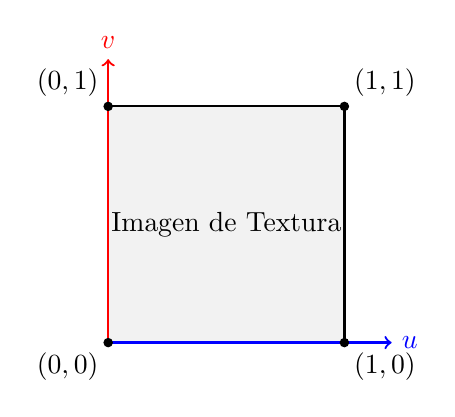
\begin{tikzpicture}[scale=3]
        % Dibujo de una cara cuadrada representando la textura
        \draw[thick, fill=gray!10] (0,0) rectangle (1,1);
        
        % Ejes UV
        \draw[->, thick, blue] (0,0) -- (1.2,0) node[right] {$u$};
        \draw[->, thick, red] (0,0) -- (0,1.2) node[above] {$v$};
        
        % Puntos
        \filldraw (0,0) circle (0.5pt) node[below left] {$(0,0)$};
        \filldraw (1,0) circle (0.5pt) node[below right] {$(1,0)$};
        \filldraw (1,1) circle (0.5pt) node[above right] {$(1,1)$};
        \filldraw (0,1) circle (0.5pt) node[above left] {$(0,1)$};
        
        % Texto explicativo
        \node at (0.5, 0.5) {Imagen de Textura};
    \end{tikzpicture}
    \end{center}

    \item \textbf{Tablas de Definición del Modelo:}
    Definiremos los vértices cara por cara. Asumiremos el orden de vértices estándar para formar dos triángulos (por ejemplo: 0-1-2 y 0-2-3 para un quad) en sentido antihorario (CCW).
\end{enumerate}



\begin{table}[H]
\centering
\small
\begin{tabular}{|c|c|c|c|}
\hline
\textbf{Cara} & \textbf{Índice ($i$)} & \textbf{Posición $(x, y, z)$} & \textbf{Coord. Textura $(u, v)$} \\
\hline
\hline
\multirow{4}{*}{\textbf{Frontal} ($z=1$)} 
& 0 & $(0, 0, 1)$ & $(0, 0)$ \\ 
& 1 & $(1, 0, 1)$ & $(1, 0)$ \\ 
& 2 & $(1, 1, 1)$ & $(1, 1)$ \\ 
& 3 & $(0, 1, 1)$ & $(0, 1)$ \\ 
\hline
\multirow{4}{*}{\textbf{Trasera} ($z=0$)} 
& 4 & $(1, 0, 0)$ & $(0, 0)$ \\ 
& 5 & $(0, 0, 0)$ & $(1, 0)$ \\ 
& 6 & $(0, 1, 0)$ & $(1, 1)$ \\ 
& 7 & $(1, 1, 0)$ & $(0, 1)$ \\ 
\hline
\multirow{4}{*}{\textbf{Derecha} ($x=1$)} 
& 8 & $(1, 0, 1)$ & $(0, 0)$ \\ 
& 9 & $(1, 0, 0)$ & $(1, 0)$ \\ 
& 10 & $(1, 1, 0)$ & $(1, 1)$ \\ 
& 11 & $(1, 1, 1)$ & $(0, 1)$ \\ 
\hline
\multirow{4}{*}{\textbf{Izquierda} ($x=0$)} 
& 12 & $(0, 0, 0)$ & $(0, 0)$ \\ 
& 13 & $(0, 0, 1)$ & $(1, 0)$ \\ 
& 14 & $(0, 1, 1)$ & $(1, 1)$ \\ 
& 15 & $(0, 1, 0)$ & $(0, 1)$ \\ 
\hline
\multirow{4}{*}{\textbf{Superior} ($y=1$)} 
& 16 & $(0, 1, 1)$ & $(0, 0)$ \\ 
& 17 & $(1, 1, 1)$ & $(1, 0)$ \\ 
& 18 & $(1, 1, 0)$ & $(1, 1)$ \\ 
& 19 & $(0, 1, 0)$ & $(0, 1)$ \\ 
\hline
\multirow{4}{*}{\textbf{Inferior} ($y=0$)} 
& 20 & $(0, 0, 0)$ & $(0, 0)$ \\ 
& 21 & $(1, 0, 0)$ & $(1, 0)$ \\ 
& 22 & $(1, 0, 1)$ & $(1, 1)$ \\ 
& 23 & $(0, 0, 1)$ & $(0, 1)$ \\ 
\hline
\end{tabular}
\caption{Tabla Combinada de Vértices y Coordenadas de Textura}
\end{table}

\vspace{0.3cm}
\textit{Nota sobre la orientación:} En la cara trasera y las laterales, el orden de los vértices y la asignación de $(u,v)$ se ha elegido para mantener la coherencia visual (que la imagen no se vea ''espejada'') y el orden de los vértices (winding order) sea consistente para el ''culling'' de caras traseras.

El código GDScript para definir las tablas de vértices y coordenadas de textura es el siguiente:
\begin{lstlisting}[language=gdscript]
# Tabla de posiciones (24 vértices: 6 caras x 4 vértices)
var vertices = [
    # Frontal (z=1)
    Vector3(0,0,1), Vector3(1,0,1), Vector3(1,1,1), Vector3(0,1,1),
    # Trasera (z=0)
    Vector3(1,0,0), Vector3(0,0,0), Vector3(0,1,0), Vector3(1,1,0),
    # Derecha (x=1)
    Vector3(1,0,1), Vector3(1,0,0), Vector3(1,1,0), Vector3(1,1,1),
    # Izquierda (x=0)
    Vector3(0,0,0), Vector3(0,0,1), Vector3(0,1,1), Vector3(0,1,0),
    # Superior (y=1)
    Vector3(0,1,1), Vector3(1,1,1), Vector3(1,1,0), Vector3(0,1,0),
    # Inferior (y=0)
    Vector3(0,0,0), Vector3(1,0,0), Vector3(1,0,1), Vector3(0,0,1),
]

# Tabla de coordenadas de textura (UV)
var uvs = [
    # Frontal
    Vector2(0,0), Vector2(1,0), Vector2(1,1), Vector2(0,1),
    # Trasera
    Vector2(0,0), Vector2(1,0), Vector2(1,1), Vector2(0,1),
    # Derecha
    Vector2(0,0), Vector2(1,0), Vector2(1,1), Vector2(0,1),
    # Izquierda
    Vector2(0,0), Vector2(1,0), Vector2(1,1), Vector2(0,1),
    # Superior
    Vector2(0,0), Vector2(1,0), Vector2(1,1), Vector2(0,1),
    # Inferior
    Vector2(0,0), Vector2(1,0), Vector2(1,1), Vector2(0,1),
]

# Tabla de triángulos 
var triangles = [
    # Frontal
    0,1,2, 0,2,3,
    # Trasera
    4,5,6, 4,6,7,
    # Derecha
    8,9,10, 8,10,11,
    # Izquierda
    12,13,14, 12,14,15,
    # Superior
    16,17,18, 16,18,19,
    # Inferior
    20,21,22, 20,22,23,
]
\end{lstlisting}

\end{solucion}

\section{Sesión 9}

\begin{ejercicio}
En una aplicación Godot cualquiera, añade código al nodo raíz de forma que cada vez que se pulse y luego se levante una tecla (por ejemplo la tecla P), se imprima en pantalla un mensaje con el tiempo total en segundos que dicha tecla ha estado pulsada, en los casos en los que ha permanecido pulsada al menos el tiempo de un frame.
\end{ejercicio}

\begin{solucion}

Para resolver este problema, debemos comprender cómo funciona el ciclo de vida de un videojuego o aplicación gráfica interactiva en tiempo real. No basta con saber que una tecla ha sido pulsada; necesitamos cuantificar la duración temporal de ese estado.

En Godot, la función \texttt{\_process(delta)} se ejecuta en cada fotograma (frame). El parámetro \texttt{delta} representa el tiempo transcurrido (en segundos) desde el fotograma anterior. Por lo tanto, la estrategia consiste en acumular este valor \texttt{delta} mientras la tecla esté presionada y, en el momento exacto en que se libera, mostrar el total acumulado.

A continuación, se presenta el diagrama de flujo lógico que seguiremos para implementar el algoritmo:

\begin{center}
\begin{tikzpicture}[node distance=2cm, every node/.style={font=\small}]

% --- ESTILOS CORREGIDOS (Se añade align=center para permitir saltos de línea \\) ---
\tikzstyle{startstop} = [rectangle, rounded corners, minimum width=2.5cm, minimum height=1cm, align=center, draw=black, fill=red!30]
\tikzstyle{io} = [trapezium, trapezium left angle=70, trapezium right angle=110, minimum width=2.5cm, minimum height=1cm, align=center, draw=black, fill=blue!30]
\tikzstyle{process} = [rectangle, minimum width=2.5cm, minimum height=1cm, align=center, draw=black, fill=orange!30]
\tikzstyle{decision} = [diamond, aspect=2, minimum width=2.5cm, minimum height=1cm, align=center, draw=black, fill=green!30, inner sep=0pt]
\tikzstyle{arrow} = [thick,->,>=stealth]

% --- NODOS ---
\node (start) [startstop] {\_process(delta)};

\node (dec1) [decision, below=of start] {¿Tecla 'P'\\pulsada?};

% Movemos proc1 a la derecha
\node (proc1) [process, right=3.5cm of dec1] {tiempo += delta};

\node (dec2) [decision, below=of dec1] {¿Estaba pulsada\\antes?};

\node (io1) [io, below=of dec2] {Imprimir tiempo};

\node (reset) [process, below=of io1] {Resetear tiempo};

% --- FLECHAS Y CONEXIONES ---

% 1. Flujo inicial
\draw [arrow] (start) -- (dec1);

% 2. Decisión 1: SI (Derecha y vuelta arriba)
\draw [arrow] (dec1) -- node[anchor=south] {Sí} (proc1); 
\draw [arrow] (proc1) |- (start); 

% 3. Decisión 1: NO (Abajo)
\draw [arrow] (dec1) -- node[anchor=east] {No} (dec2);

% 4. Decisión 2: NO (Izquierda y vuelta arriba - Bucle ''Idle'')
\draw [arrow] (dec2.west) -- ++(-2.5,0) |- (start.west);
\node[anchor=south east] at ($(dec2.west) + (-0.2,0)$) {No};

% 5. Decisión 2: SI (Abajo - Soltada)
\draw [arrow] (dec2) -- node[anchor=east] {Sí (Soltada)} (io1);
\draw [arrow] (io1) -- (reset);

% 6. Retorno final (Desde Reset hasta Start por la izquierda exterior)
\draw [arrow] (reset.west) -- ++(-3.5,0) |- (start.west);

\end{tikzpicture}
\end{center}

\vspace{0.5cm}

\textbf{Implementación paso a paso:}

\begin{enumerate}
\item \textbf{Definición de variables de estado:}
Necesitamos una variable para acumular el tiempo (\texttt{tiempo\_pulsado}) y una variable booleana (\texttt{tecla\_activa}) para saber si estamos en medio de una acción de pulsación. Esto es necesario para detectar el evento ''just released'' (acaba de ser soltada) manualmente o mediante la lógica de estados.

\item \textbf{Uso del bucle de procesamiento:}
Utilizaremos la función virtual \texttt{\_process(delta)}, que Godot invoca continuamente.

\item \textbf{Lógica de entrada (Input):}
Usaremos la clase \texttt{Input} para sondear (polling) el estado físico de la tecla 'P' (código \texttt{KEY\_P}).

\item \textbf{Acumulación y Reporte:}
\begin{itemize}
    \item Si la tecla está pulsada: Sumamos \texttt{delta} a nuestra variable acumuladora.
    \item Si la tecla NO está pulsada pero \texttt{tecla\_activa} es verdadera: Significa que el usuario acaba de soltar la tecla. En ese momento imprimimos el valor y reiniciamos las variables.
\end{itemize}

\end{enumerate}

\vspace{0.5cm}

\textbf{Código GDScript Solución:}

\begin{lstlisting}
extends Node

# Variable para almacenar el tiempo acumulado en segundos

var tiempo_acumulado: float = 0.0

# Bandera para controlar el estado de la tecla (si se está manteniendo pulsada)

var tecla_esta_pulsada: bool = false

func _process(delta: float) -> void:
# Verificamos si la tecla P está siendo presionada en este frame
if Input.is_key_pressed(KEY_P):
# Marcamos que la tecla está activa
tecla_esta_pulsada = true

    # Acumulamos el tiempo transcurrido desde el último frame
    tiempo_acumulado += delta
    
else:
    # Si la tecla NO está pulsada, verificamos si lo estaba en el frame anterior
    # Esto indica el evento ''Just Released'' (Acaba de soltarse)
    if tecla_esta_pulsada:
        
        # Verificamos la condición del enunciado: 
        # ''permanecido pulsada al menos el tiempo de un frame''
        # Si tiempo_acumulado > 0, significa que al menos un frame sumó delta.
        if tiempo_acumulado > 0.0:
            print(''La tecla P se mantuvo pulsada durante: '', 
                  tiempo_acumulado, '' segundos.'')
        
        # Reiniciamos el estado para la próxima pulsación
        tiempo_acumulado = 0.0
        tecla_esta_pulsada = false

\end{lstlisting}

\end{solucion}

\begin{ejercicio}
Una posibilidad para hacer selección en mallas de triángulos es usar cálculo
de intersecciones entre un rayo (una semirrecta que pasa por el centro de un
píxel) y cada uno de los triángulos de la malla. 

Diseña un algoritmo en pseudo-código para el cálculo de intersecciones entre un rayo y un triángulo:

\begin{itemize}
    \item El rayo tiene como origen o extremo el punto cuyas coordenadas del mundo es la tupla $\mathbf{o}$, y como vector de dirección la tupla $\mathbf{d}$ (la suponemos normalizada).
    \item Las coordenadas del mundo de los vértices del triángulo son $\mathbf{v}_0$, $\mathbf{v}_1$ y $\mathbf{v}_2$.
    \item El algoritmo debe indicar si hay intersección o no, y, en caso de que la haya, calcular las coordenadas del mundo del punto de intersección.
\end{itemize}

%Diseña un algoritmo en pseudo-código para el cálculo de intersecciones entre un rayo y un triángulo. 

Ten en cuenta que habrá intersección si y solo si se cumplen cada una de estas
dos condiciones:

\begin{itemize}
    \item El rayo intersecta con el plano del triángulo si y solo si existe $t > 0$ tal que el punto $p_t = o + t d$ está en el plano. Esto equivale a que el vector $p_t - v_0$ es perpendicular a la normal del plano $n$ (es decir, su producto escalar es nulo).
    \item El punto $p_t$ está dentro del triángulo si existen dos valores reales no negativos $a$ y $b$ (con $0 \leq a + b \leq 1$) tales que el vector $p_t - v_0 = a (v_1 - v_0) + b (v_2 - v_0)$. A los tres valores $a$, $b$ y $c \equiv 1 - a - b$ se les llama coordenadas baricéntricas de $p_t$ en el triángulo.
\end{itemize}

\begin{center}
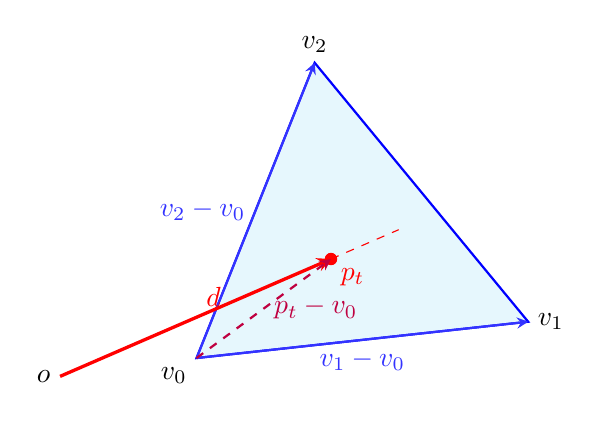
\begin{tikzpicture}[scale=1.5, >=stealth]
% Coordenadas
\coordinate (O) at (0, 1, 3); % Origen rayo
\coordinate (V0) at (0, 0, 0);
\coordinate (V1) at (3, 0.5, 0.5);
\coordinate (V2) at (1, 2.5, 0);
\coordinate (Pt) at (1.2, 0.9, 0.16); % Punto intersección aproximado


% Triángulo
\filldraw[fill=cyan!10, draw=blue, thick] (V0) -- (V1) -- (V2) -- cycle;

% Vectores aristas
\draw[->, blue!80, thick] (V0) -- (V1) node[midway, below] {$v_1 - v_0$};
\draw[->, blue!80, thick] (V0) -- (V2) node[midway, left] {$v_2 - v_0$};

% Rayo
\draw[->, red, very thick] (O) -- (Pt) node[midway, above right] {$d$};
\draw[red, dashed] (Pt) -- (1.5, 0.875, -0.55);

% Puntos y etiquetas
\node[below left] at (V0) {$v_0$};
\node[right] at (V1) {$v_1$};
\node[above] at (V2) {$v_2$};
\node[left] at (O) {$o$};
\fill[red] (Pt) circle (1.5pt) node[below right] {$p_t$};

% Vector w
\draw[->, purple, dashed, thick] (V0) -- (Pt) node[midway, right] {$p_t - v_0$};



\end{tikzpicture}
\end{center}
\end{ejercicio}

\begin{solucion}
Para resolver el problema siguiendo estrictamente las condiciones dadas, el algoritmo se estructura en dos fases secuenciales: encontrar el punto en el plano (Condición 1) y validar si dicho punto está contenido en la región triangular (Condición 2).

\textbf{Procedimiento detallado:}

\begin{enumerate}
\item \textbf{Cálculo de la Normal del Plano:}
Primero, definimos los vectores directores del plano del triángulo basándonos en sus aristas:
$$
e_1 = v_1 - v_0
$$
$$
e_2 = v_2 - v_0
$$

La normal $n$ se obtiene mediante el producto vectorial:
$$
n = e_1 \times e_2
$$


\item \textbf{Condición 1: Intersección con el Plano:}
Buscamos un $t$ tal que el vector desde $v_0$ hasta el punto de impacto $p_t$ sea ortogonal a la normal.
La ecuación del plano es $(p - v_0) \cdot n = 0$.
Sustituyendo la ecuación del rayo $p = o + t \cdot d$:
$$((o + t \cdot d) - v_0) \cdot n = 0$$
$$(o - v_0) \cdot n + t(d \cdot n) = 0$$
Despejando $t$:
$$t = \frac{(v_0 - o) \cdot n}{d \cdot n}$$
Si $d \cdot n \approx 0$, el rayo es paralelo al plano (no hay intersección). Si $t \leq 0$, el triángulo está detrás del origen. 

\item \textbf{Condición 2: Inclusión en el Triángulo (Coordenadas Baricéntricas):}
Una vez tenemos $p_t = o + t \cdot d$, definimos el vector $w = p_t - v_0$. Según el enunciado, debemos encontrar $a$ y $b$ tales que:
$$w = a \cdot e_1 + b \cdot e_2$$
Esto es un sistema de ecuaciones lineales. Para resolverlo eficientemente usando productos escalares, multiplicamos la ecuación por $e_1$ y por $e_2$:
\begin{enumerate}
    \item $(w \cdot e_1) = a(e_1 \cdot e_1) + b(e_2 \cdot e_1)$
    \item $(w \cdot e_2) = a(e_1 \cdot e_2) + b(e_2 \cdot e_2)$
\end{enumerate}
Aplicando la regla de Cramer para despejar $a$ y $b$:
$$a = \frac{(w \cdot e_1)(e_2 \cdot e_2) - (w \cdot e_2)(e_1 \cdot e_2)}{(e_1 \cdot e_1)(e_2 \cdot e_2) - (e_1 \cdot e_2)^2}$$
$$b = \frac{(e_1 \cdot e_1)(w \cdot e_2) - (e_1 \cdot e_2)(w \cdot e_1)}{(e_1 \cdot e_1)(e_2 \cdot e_2) - (e_1 \cdot e_2)^2}$$
Finalmente, verificamos si $a \geq 0$, $b \geq 0$ y $a + b \leq 1$.



\end{enumerate}

\vspace{0.5cm}

\textbf{Algoritmo en Pseudo-código:}

\begin{lstlisting}[language=C++,  frame=single, numbers=left, breaklines=true, keywordstyle=\color{blue}, commentstyle=\color{green!60!black}, stringstyle=\color{purple}]
Funcion IntersectarRayoTriangulo(o, d, v0, v1, v2):
// --- Pre-computo de vectores del triangulo ---
Vector3 e1 = v1 - v0
Vector3 e2 = v2 - v0
Vector3 n  = ProductoCruz(e1, e2) // Normal del plano


// --- Condicion 1: Interseccion Rayo-Plano ---

// Calculamos el denominador (d . n)
float det = ProductoPunto(d, n)

// Si es cercano a 0, el rayo es paralelo al triangulo
Si valor_absoluto(det) < EPSILON:
    Retornar {Falso, Nulo}

// Calculamos t usando la formula derivada: t = ((v0 - o) . n) / det
Vector3 origen_a_v0 = v0 - o
float t = ProductoPunto(origen_a_v0, n) / det

// Verificamos que la interseccion esta delante de la camara (t > 0)
Si t < EPSILON:
    Retornar {Falso, Nulo}

// Calculamos el punto de interseccion en el plano
Vector3 pt = o + (d * t)

// --- Condicion 2: Punto dentro del triangulo ---
// Debemos resolver: pt - v0 = a*e1 + b*e2

Vector3 w = pt - v0 

// Calculo de productos punto para el sistema de Cramer
float uu = ProductoPunto(e1, e1)
float uv = ProductoPunto(e1, e2)
float vv = ProductoPunto(e2, e2)
float wu = ProductoPunto(w, e1)
float wv = ProductoPunto(w, e2)

// Denominador del sistema (determinante)
float denominador = (uu * vv) - (uv * uv)

// Si denominador es 0, el triangulo es degenerado (linea o punto)
Si valor_absoluto(denominador) < EPSILON:
    Retornar {Falso, Nulo}

// Calculo de coordenadas baricentricas a y b
float a = ((wu * vv) - (wv * uv)) / denominador
float b = ((uu * wv) - (wu * uv)) / denominador

// Verificacion final de limites baricentricos
// 0 <= a, 0 <= b, a + b <= 1
Si (a >= 0.0) Y (b >= 0.0) Y (a + b <= 1.0):
    Retornar {Verdadero, pt}
Sino:
    Retornar {Falso, Nulo}



\end{lstlisting}
\end{solucion}

\begin{solucion} Otra resolución alternativa y más detallada es la que se proporciona a continuación.
Para resolver este problema, debemos traducir la geometría 3D a una serie de pasos lógicos. No basta con aplicar fórmulas; hay que entender qué significan. El proceso se divide en tres fases: definir la pared (plano), buscar el choque y verificar si el choque está dentro del triángulo.

\subsubsection*{1. Definición del Plano (La Pared)}
Un triángulo es plano. Para saber si un rayo choca con él, primero necesitamos saber la orientación de la pared invisible donde está pegado el triángulo.
\begin{itemize}
    \item Calculamos dos vectores que bordean el triángulo desde $\mathbf{v}_0$:
    $$ \mathbf{e}_1 = \mathbf{v}_1 - \mathbf{v}_0, \quad \mathbf{e}_2 = \mathbf{v}_2 - \mathbf{v}_0 $$
    \item La orientación (el vector normal $\mathbf{n}$) es perpendicular a ambos bordes:
    $$ \mathbf{n} = \mathbf{e}_1 \times \mathbf{e}_2 $$
\end{itemize}

\subsubsection*{2. El Choque (Cálculo de $t$)}
El rayo es una línea que empieza en $\mathbf{o}$ y avanza en dirección $\mathbf{d}$. La fórmula del impacto en el plano es:
$$ t = \frac{(\mathbf{v}_0 - \mathbf{o}) \cdot \mathbf{n}}{\mathbf{d} \cdot \mathbf{n}} $$

\textbf{¿Por qué $t < 0$ significa ``detrás''?}
Imagina que el rayo son tus pasos.
\begin{itemize}
    \item $\mathbf{t=0}$ es donde estás parado (el origen).
    \item $\mathbf{t>0}$ son pasos hacia adelante (lo que ves).
    \item $\mathbf{t<0}$ son pasos hacia atrás (a tu espalda).
\end{itemize}
La fórmula matemática asume una recta infinita (hacia adelante y atrás). Si el cálculo da $t = -5$, significa que el plano está 5 pasos a tu espalda. Como una cámara solo "ve" hacia adelante, descartamos cualquier $t < 0$.

\subsubsection*{3. ¿Dentro o Fuera? (Coordenadas Baricéntricas)}
Si $t > 0$, el rayo golpea la pared en el punto $\mathbf{p}$. Ahora usamos coordenadas baricéntricas ($a, b$) para ver si ese punto cae dentro del dibujo del triángulo. Es como preguntar: \textit{"¿Puedo llegar al punto $\mathbf{p}$ dando pasos solo a lo largo de los bordes $\mathbf{e}_1$ y $\mathbf{e}_2$ sin salirme?"}.

Se resuelve el sistema $\mathbf{p} - \mathbf{v}_0 = a \mathbf{e}_1 + b \mathbf{e}_2$. Si $a \geq 0$, $b \geq 0$ y $a+b \leq 1$, estamos dentro.

\vspace{0.5cm}

\begin{algorithm}[H]
\caption{Intersección Rayo-Triángulo}
\begin{algorithmic}[1]
\State \textbf{Entrada:} Rayo ($\mathbf{o}, \mathbf{d}$), Triángulo ($\mathbf{v}_0, \mathbf{v}_1, \mathbf{v}_2$)
\State \textbf{Salida:} Bool (¿Impacto?), Punto ($\mathbf{p}$)

\Statex \Comment{--- Fase 1: Preparar vectores ---}
\State $\mathbf{e}_1 \gets \mathbf{v}_1 - \mathbf{v}_0$
\State $\mathbf{e}_2 \gets \mathbf{v}_2 - \mathbf{v}_0$
\State $\mathbf{n} \gets \mathbf{e}_1 \times \mathbf{e}_2$ \Comment{Producto Vectorial (Normal)}

\Statex \Comment{--- Fase 2: Intersección con el plano ---}
\State $det \gets \mathbf{d} \cdot \mathbf{n}$
\If{$|det| < \epsilon$} \Comment{¿Es el rayo paralelo al plano?}
    \State \Return \textbf{Falso}, Nulo
\EndIf

\State $\mathbf{vec\_origen} \gets \mathbf{v}_0 - \mathbf{o}$
\State $t \gets (\mathbf{vec\_origen} \cdot \mathbf{n}) / det$

\If{$t < 0$} \Comment{Si t es negativo, el triángulo está detrás}
    \State \Return \textbf{Falso}, Nulo
\EndIf

\Statex \Comment{--- Fase 3: Test de inclusión (Baricéntricas) ---}
\State $\mathbf{p} \gets \mathbf{o} + (t \cdot \mathbf{d})$ \Comment{Punto de impacto en el plano}
\State $\mathbf{w} \gets \mathbf{p} - \mathbf{v}_0$

\Statex \Comment{Resolvemos sistema lineal usando prod. escalares (Cramer)}
\State $uu \gets \mathbf{e}_1 \cdot \mathbf{e}_1; \quad uv \gets \mathbf{e}_1 \cdot \mathbf{e}_2; \quad vv \gets \mathbf{e}_2 \cdot \mathbf{e}_2$
\State $wu \gets \mathbf{w} \cdot \mathbf{e}_1; \quad wv \gets \mathbf{w} \cdot \mathbf{e}_2$
\State $D \gets (uu \cdot vv) - (uv \cdot uv)$

\State $a \gets ((wu \cdot vv) - (wv \cdot uv)) / D$
\State $b \gets ((uu \cdot wv) - (uv \cdot wu)) / D$

\If{$a \geq 0 \land b \geq 0 \land (a + b \leq 1)$}
    \State \Return \textbf{Verdadero}, $\mathbf{p}$ \Comment{¡Impacto confirmado!}
\Else
    \State \Return \textbf{Falso}, Nulo \Comment{Fuera del triángulo}
\EndIf
\end{algorithmic}
\end{algorithm}
\hspace{1cm}

\end{solucion}

\begin{ejercicio}
Para implementar la selección usando intersecciones es necesario calcular el rayo que tiene como origen el observador y pasa por el centro del pixel donde se ha hecho click.

Escribe el pseudo-código del algoritmo que calcula el rayo a partir de las coordenadas del pixel donde se ha hecho click:
\begin{itemize}
\item Tenemos una vista perspectiva, y conocemos los 6 valores  usados para construir la matriz de proyección (left, right, top, bottom, near, far).
\item También conocemos el marco de coordenadas de vista, es decir, las tuplas  y  con los versores y la tupla  con el punto origen (todos en coordenadas del mundo).
\item El viewport tiene  columnas y  filas de pixels.
\item Se ha hecho click en el pixel de coordenadas enteras  e .
\end{itemize}
El algoritmo debe producir como salida las tuplas  y  (normalizado) que definen el rayo.

\begin{center}
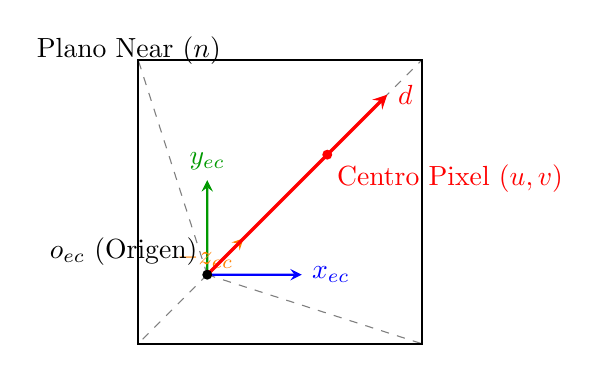
\begin{tikzpicture}[scale=1.2, >=stealth]
% Sistema de coordenadas de la cámara (Eye Coordinates)
\coordinate (Oec) at (0, 0, 4);


% Plano de imagen (Near Plane)
\coordinate (TL) at (-1.5, 1.5, 2); % Top-Left
\coordinate (TR) at (1.5, 1.5, 2);  % Top-Right
\coordinate (BL) at (-1.5, -1.5, 2); % Bottom-Left
\coordinate (BR) at (1.5, -1.5, 2);  % Bottom-Right

% Pixel clickado (representado en el plano near)
\coordinate (Pixel) at (0.5, 0.5, 2);

% Ejes de la cámara
\draw[->, thick, blue] (Oec) -- (1, 0, 4) node[right] {$x_{ec}$};
\draw[->, thick, green!60!black] (Oec) -- (0, 1, 4) node[above] {$y_{ec}$};
\draw[->, thick, orange] (Oec) -- (0, 0, 3) node[below left] {$-z_{ec}$};

% Dibujar pirámide de visión (Frustum truncado visualmente)
\draw[dashed, gray] (Oec) -- (TL);
\draw[dashed, gray] (Oec) -- (TR);
\draw[dashed, gray] (Oec) -- (BL);
\draw[dashed, gray] (Oec) -- (BR);

% Plano Near
\draw[thick, black] (TL) -- (TR) -- (BR) -- (BL) -- cycle;
\node at (-1.6, 1.6, 2) {Plano Near ($n$)};

% Rayo
\draw[->, red, very thick] (Oec) -- (Pixel) -- (0.75, 0.75, 1) node[right] {$d$};
\fill[red] (Pixel) circle (1.5pt) node[below right] {Centro Pixel ($u, v$)};
\fill[black] (Oec) circle (1.5pt) node[above left] {$o_{ec}$ (Origen)};



\end{tikzpicture}
\end{center}
\end{ejercicio}

\begin{solucion}

El objetivo de este ejercicio es realizar el proceso inverso a la rasterización: en lugar de proyectar un punto 3D a un pixel 2D, queremos proyectar un pixel 2D hacia el espacio 3D (''Un-project'').

Para ello, debemos transformar las coordenadas del pixel  desde el espacio de pantalla al espacio de la cámara (View Space), y finalmente rotar ese vector al espacio del mundo (World Space) usando la base de la cámara dada.

\textbf{Procedimiento paso a paso:}

\begin{enumerate}
\item \textbf{Mapeo de Pixel a Plano de Imagen (View Plane):}
El plano de proyección se encuentra a una distancia  (near) de la cámara. Los límites de este plano son  en horizontal y  en vertical.


Los pixels se indexan generalmente desde la esquina superior izquierda $(0,0)$ hasta $(w, filas)$. Sin embargo, el sistema de coordenadas de la cámara suele tener el eje $Y$ apuntando hacia arriba. Debemos tener cuidado con esta inversión.

Calculamos las coordenadas físicas $(u, v)$ en el plano near correspondientes al centro del pixel:
\begin{itemize}
    \item Sumamos $0.5$ a $x_p$ y $y_p$ para apuntar al \textit{centro} del pixel, no a su esquina.
    \item Interpolamos linealmente:
    $$u = l + (r - l) \cdot \frac{x_p + 0.5}{w}$$
    $$v = t - (t - b) \cdot \frac{y_p + 0.5}{filas}$$
    \textit{Nota: Asumimos que $y_p=0$ es la parte superior (top) y $y_p=filas$ es la inferior (bottom), por eso restamos en $v$.}
\end{itemize}

\item \textbf{Construcción del Vector en Espacio de Cámara:}
En el sistema de referencia local de la cámara:
\begin{itemize}
    \item El origen del rayo es $(0,0,0)$.
    \item El rayo atraviesa el plano near en $(u, v, -n)$. (Recordemos que en OpenGL/Godot la cámara mira hacia $-Z$).
    \item El vector dirección local es $\vec{d}_{local} = (u, v, -n)$.
\end{itemize}

\item \textbf{Transformación al Espacio del Mundo:}
Ahora usamos la base de la cámara dada ($x_{ec}, y_{ec}, z_{ec}$) para orientar este vector en el mundo. 
$$\vec{d}_{mundo} = u \cdot \vec{x}_{ec} + v \cdot \vec{y}_{ec} + (-n) \cdot \vec{z}_{ec}$$

El origen del rayo $o$ es simplemente la posición de la cámara $o_{ec}$.

\item \textbf{Normalización:}
Finalmente, normalizamos el vector dirección resultante.



\end{enumerate}

\vspace{0.5cm}

\textbf{Algoritmo en Pseudo-código:}

\begin{lstlisting}[language=C++,  frame=single, numbers=left, breaklines=true, keywordstyle=\color{blue}, commentstyle=\color{green!60!black}, stringstyle=\color{purple}]
Funcion CalcularRayoDesdePixel(xp, yp, w, filas, l, r, b, t, n, o_ec, x_ec, y_ec, z_ec):

// 1. Calcular coordenadas normalizadas del centro del pixel (0.0 a 1.0)
// Sumamos 0.5 para tomar el centro exacto del pixel
float ratio_x = (xp + 0.5) / w
float ratio_y = (yp + 0.5) / filas

// 2. Mapear al tamaño fisico del plano near (View Plane)
// Coordenada u (horizontal): interpolar entre left (l) y right (r)
float u = l + ((r - l) * ratio_x)

// Coordenada v (vertical): interpolar entre top (t) y bottom (b)
// IMPORTANTE: Asumimos que yp=0 es arriba (top) y yp=filas es abajo (bottom)
// Por tanto, a mayor yp, nos acercamos mas a 'b' y nos alejamos de 't'
float v = t - ((t - b) * ratio_y) 

// 3. Construir el vector de direccion en coordenadas del mundo
// El vector en espacio camara es (u, v, -n)
// Lo transformamos multiplicando por los versores de la base de la camara
// d = u*Right + v*Up + (-n)*Back

Vector3 direccion_no_norm = (x_ec * u) + (y_ec * v) - (z_ec * n)

// 4. Normalizar la direccion
Vector3 d = Normalizar(direccion_no_norm)

// 5. El origen del rayo es la posicion de la camara (proyeccion perspectiva)
Vector3 o = o_ec

Retornar {o, d}



\end{lstlisting}
\end{solucion}


\section{Sesión 10}

\begin{ejercicio}

Supongamos que un rayo (una semirrecta en 3D) tiene como origen o extremo el punto cuyas coordenadas del mundo es la tupla $\mathbf{o}$, y como vector de dirección la tupla $\mathbf{d}$ (la suponemos normalizada). Además, sabemos que un disco de radio $r$ tiene como centro el punto de coordenadas de mundo $\mathbf{c}$ y está en el plano perpendicular al vector $\mathbf{n}$.

Con estos datos de entrada, diseña un algoritmo para calcular si hay intersección entre el rayo y el disco.

Ten en cuenta que habrá intersección si y solo si se cumplen cada
una de estas dos condiciones:
\begin{enumerate}
    \item El rayo interseca con el plano que contiene al disco, es
    decir, existe $t > 0$ tal que el punto $p_t \equiv o + t d$ está en dicho
    plano. Equivale a decir que el vector $p_t - c$ es perpendicular a
    la normal al plano $n$.
    \item El punto $p_t$ citado arriba está dentro del disco, es decir, su
    distancia a $c$ es inferior al radio.
\end{enumerate}
% \vspace{0.5cm}
% \centering
% \begin{tikzpicture}[scale=1.2]
% % Definición de coordenadas para simular 3D
% \coordinate (O) at (-2, 2); % Origen del rayo
% \coordinate (C) at (2, 0);  % Centro del disco
% \coordinate (P) at (1, 0.5); % Punto de intersección aproximado


% % Dibujo del plano (perspectiva)
% \draw[fill=gray!10, dashed] (-1, -1.5) -- (4, -1.5) -- (5, 2.5) -- (0, 2.5) -- cycle;
% \node at (4.5, 2.2) {Plano $\pi$};

% % Dibujo del disco
% \draw[fill=blue!20, opacity=0.8] (C) ellipse (1.5 and 0.8);
% \node[below right] at (C) {$c$ (centro)};
% \fill (C) circle (1.5pt);

% % Vector Normal
% \draw[->, thick, red] (C) -- ++(0, 1.5) node[above] {$n$};

% % Rayo (parte visible antes del plano)
% \draw[->, thick, black] (O) -- (P);
% \fill (O) circle (1.5pt) node[left] {$o$ (origen)};
% \node[above] at (-0.5, 1.25) {$d$};

% % Intersección
% \fill[red] (P) circle (1.5pt) node[right, yshift=-0.2cm] {$p_t$ (intersección)};

% % Rayo (proyección imaginaria)
% \draw[dashed] (P) -- ++(1, -0.33);

% % Radio
% \draw[<->, thin] (C) -- ++(1.5, 0) node[midway, below] {$r$};

% % Vector p - c
% \draw[->, blue, thick] (C) -- (P) node[midway, above left, scale=0.7] {$p_t - c$};



% \end{tikzpicture}
\end{ejercicio}

\begin{solucion}
Para resolver este problema geométrico fundamental en el trazado de rayos (\textit{ray-tracing}), se debe descomponer la situación en dos etapas lógicas secuenciales. Primero, se determina el punto donde el rayo infinito cruza el plano matemático que contiene al disco. Segundo, se verifica si dicho punto de cruce se encuentra dentro de los límites finitos del disco (es decir, dentro de su radio).

\begin{enumerate}
\item \textbf{Definición Algebraica del Rayo y el Plano:}


Un rayo se define paramétricamente como una línea que parte de un origen $o$ y avanza en la dirección $d$. Cualquier punto $p(t)$ sobre el rayo se puede expresar como:
$$p(t) = o + t \cdot d$$
Donde $t$ es un escalar real ($t \ge 0$) que representa la distancia desde el origen a lo largo del vector dirección.

Por otro lado, un plano en el espacio 3D queda definido por un punto conocido (en este caso, el centro del disco $c$) y un vector normal $n$ perpendicular a la superficie. La condición para que un punto genérico $p$ pertenezca al plano es que el vector formado entre el centro y ese punto sea perpendicular a la normal. Matemáticamente, esto implica que su producto escalar (\textit{dot product}) es cero:
$$(p - c) \cdot n = 0$$

\item \textbf{Cálculo del parámetro de intersección $t$:}

Para encontrar la intersección, se sustituye la ecuación del rayo en la ecuación del plano:
$$((o + t \cdot d) - c) \cdot n = 0$$

Aplicando la propiedad distributiva del producto escalar:
$$(o - c) \cdot n + (t \cdot d) \cdot n = 0$$
$$(o \cdot n) - (c \cdot n) + t(d \cdot n) = 0$$

Despejando $t$:
$$t(d \cdot n) = (c \cdot n) - (o \cdot n)$$
$$t(d \cdot n) = (c - o) \cdot n$$
$$t = \frac{(c - o) \cdot n}{d \cdot n}$$

Aquí surgen consideraciones críticas de implementación:
\begin{itemize}
    \item Si el denominador $d \cdot n$ es igual a 0, significa que el rayo es perpendicular a la normal del plano (es decir, el rayo es paralelo al plano), por lo que no hay intersección (o el rayo está contenido en el plano).
    \item Si $t < 0$, la intersección ocurre ''detrás'' del origen del rayo, por lo que no es visible y debe descartarse.
\end{itemize}

\item \textbf{Cálculo del punto de intersección $p_t$:}

Una vez obtenido un $t$ válido ($t > 0$), se calcula la coordenada exacta del punto en el espacio:
$$p_t = o + t \cdot d$$

\item \textbf{Verificación de pertenencia al disco:}

El hecho de que $p_t$ esté en el plano no garantiza que golpee el disco. Para que haya colisión, la distancia entre el punto de intersección $p_t$ y el centro del disco $c$ debe ser menor o igual al radio $r$.
$$\| p_t - c \| \le r$$

Computacionalmente, calcular la raíz cuadrada para el módulo de un vector es costoso. Es preferible comparar los cuadrados de las distancias:
$$v = p_t - c$$
$$v \cdot v \le r^2$$
$$(v_x^2 + v_y^2 + v_z^2) \le r^2$$



\end{enumerate}

A continuación, se presenta el algoritmo formal en pseudocódigo:

\begin{lstlisting}[language=C++, frame=single,  keywordstyle=\color{blue}, commentstyle=\color{green!60!black}, captionpos=b, caption={Algoritmo de Intersección Rayo-Disco}]
// Estructuras de datos:
// Vec3: tupla (x, y, z) con operaciones de suma, resta y producto punto
// Rayo: origen (Vec3), direccion (Vec3)
// Disco: centro (Vec3), normal (Vec3), radio (float)

bool IntersectaDisco(Rayo ray, Disco disco, float &t_salida) {
    // 1. Calcular el denominador (producto punto entre normal y direccion)
    float denom = dot(disco.normal, ray.direccion);


    // Si denom es cercano a 0, el rayo es paralelo al plano
    if (abs(denom) < 1e-6) {
        return false; 
    }

    // 2. Calcular el vector desde el origen del rayo al centro del disco
    Vec3 vector_origen_centro = disco.centro - ray.origen;

    // 3. Calcular t
    float t = dot(vector_origen_centro, disco.normal) / denom;

    // Verificar si la interseccion esta detras de la camara
    if (t < 0) {
        return false;
    }

    // 4. Calcular el punto exacto de interseccion en el plano
    Vec3 p = ray.origen + (ray.direccion * t);

    // 5. Verificar si el punto esta dentro del radio del disco
    Vec3 v = p - disco.centro;
    float dist_cuadrada = dot(v, v); // |v|^2

    if (dist_cuadrada <= (disco.radio * disco.radio)) {
        t_salida = t; // Guardamos la distancia a la colision
        return true;  // Hay interseccion valida
    }

    return false; // Intersecta el plano, pero fuera del disco



}
\end{lstlisting}

Otro formato del algoritmo en pseudocódigo es el siguiente:

\begin{algorithm}[H]
\caption{Intersección Rayo-Disco}
\begin{algorithmic}[1]
\Function{InterseccionRayoDisco}{o, d, c, n, r}
    \State denom $\gets$ $d \cdot n$
    \If{$|\text{denom}| < \epsilon$}
        \State \Return (\textbf{FALSO}, NULO)
    \EndIf
    \State $t \gets \frac{(c - o) \cdot n}{\text{denom}}$
    \If{$t < 0$}
        \State \Return (\textbf{FALSO}, NULO)
    \EndIf
    \State $p \gets o + t \cdot d$
    \If{$(p - c) \cdot (p - c) \leq r^2$}
        \State \Return (\textbf{VERDADERO}, $p$)
    \Else
        \State \Return (\textbf{FALSO}, NULO)
    \EndIf
\EndFunction
\end{algorithmic}
\end{algorithm}
\hspace{1cm}

\textit{Observación.} Sabemos que $\varepsilon$ es un valor muy pequeño (por ejemplo, $10^{-6}$) para evitar divisiones por cero numéricas.

\end{solucion}


\begin{ejercicio}
% \textbf{Problema 10.2: Intersección Rayo-Esfera}

Diseña un algoritmo para calcular la primera intersección entre un
rayo (con origen en $o$ y vector $d$, normalizado) y una esfera de radio
unidad y centro en el origen, si hay alguna.

Ten en cuenta que un punto cualquiera $p$ está en la esfera si y solo si el
módulo de $p$ es la unidad, es decir, si y solo si $F(p) = 0$, donde $F$ es
el campo escalar definido así:
\[
F(p) \equiv p \cdot p - 1
\]

Describe cómo podría usarse ese mismo algoritmo para calcular la
intersección con una esfera con centro y radio arbitrarios (este
problema puede reducirse al anterior si el rayo se traslada a un
espacio de coordenadas donde la esfera tiene centro en el origen y
radio unidad).

\vspace{0.5cm}
\centering
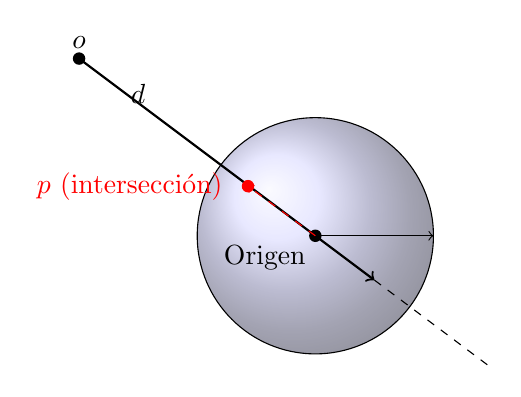
\begin{tikzpicture}[scale=1.5]
% Esfera (círculo en 2D)
\shade[ball color=blue!20, opacity=0.6] (0,0) circle (1cm);
\draw (0,0) circle (1cm);
\draw[->, thin] (0,0) -- (1,0) node[midway, below] {};
\fill (0,0) circle (1.5pt) node[below left] {Origen};

% Rayo
\coordinate (O) at (-2, 1.5);
\coordinate (D) at (0.8, -0.6); % Dirección aproximada
\draw[->, thick, black] (O) -- (0.5, -0.375); % Rayo visual
\draw[dashed] (0.5, -0.375) -- (1.5, -1.125); % Proyección

% Elementos del rayo
\fill (O) circle (1.5pt) node[above] {$o$};
\node at (-1.5, 1.2) {$d$};

% Puntos de intersección
% Intersección 1 (entrada)
\coordinate (P1) at (-0.57, 0.42); % Punto aproximado en la esfera
\fill[red] (P1) circle (1.5pt) node[left, xshift=-0.2cm] {$p$ (intersección)};

% Vector p
\draw[->, red, dashed] (0,0) -- (P1);

\end{tikzpicture}
\end{ejercicio}

\begin{solucion}
Para resolver el problema de la intersección entre un rayo y una esfera unitaria centrada en el origen, se procede algebraicamente sustituyendo la ecuación paramétrica del rayo en la ecuación implícita de la esfera. El objetivo es hallar el valor del parámetro $t$ (distancia desde el origen del rayo) donde ocurre el contacto.

\begin{enumerate}
\item \textbf{Planteamiento de las ecuaciones:}

La ecuación del rayo es:
$$p(t) = o + t \cdot d$$
donde $t \geq 0$.

La ecuación implícita de la esfera unitaria centrada en el origen es:
$$p \cdot p - 1 = 0 \quad (\text{o bien } \|p\|^2 = 1)$$

\item \textbf{Sustitución:}

Se sustituye $p(t)$ en la ecuación de la esfera:
$$(o + t \cdot d) \cdot (o + t \cdot d) - 1 = 0$$

Expandiendo el producto escalar (propiedad distributiva):
$$(o \cdot o) + 2t(o \cdot d) + t^2(d \cdot d) - 1 = 0$$

\item \textbf{Simplificación:}

Dado que el vector de dirección $d$ está normalizado, sabemos que $d \cdot d = 1$. La ecuación se convierte en una ecuación cuadrática de la forma $At^2 + Bt + C = 0$:
$$t^2 + 2(o \cdot d)t + (o \cdot o - 1) = 0$$

Identificamos los coeficientes:
\begin{itemize}
    \item $A = 1$
    \item $B = 2(o \cdot d)$
    \item $C = o \cdot o - 1$
\end{itemize}

\item \textbf{Resolución de la ecuación cuadrática:}
\hspace{1cm}
\textit{Observación.} Aunque la resolución sea trivial, se detalla

Usamos la fórmula general para hallar $t$:
$$t = \frac{-B \pm \sqrt{B^2 - 4AC}}{2A}$$

Sustituyendo $A=1$, $B=2(o \cdot d)$, $C=o \cdot o - 1$:
$$t = \frac{-2(o \cdot d) \pm \sqrt{4(o \cdot d)^2 - 4(o \cdot o - 1)}}{2}$$
$$t = -(o \cdot d) \pm \sqrt{(o \cdot d)^2 - (o \cdot o - 1)}$$

\item \textbf{Interpretación del discriminante ($\Delta$):}

El término dentro de la raíz es el discriminante: $\Delta = (o \cdot d)^2 - (o \cdot o - 1)$.
\begin{itemize}
    \item Si $\Delta < 0$: El rayo no toca la esfera (pasa de largo). No hay solución real.
    \item Si $\Delta = 0$: El rayo es tangente a la esfera (un punto de contacto).
    \item Si $\Delta > 0$: El rayo atraviesa la esfera (dos puntos de contacto, entrada y salida).
\end{itemize}
Se busca la \textbf{primera intersección}, que corresponde al menor valor positivo de $t$. Si ambos $t$ son negativos, la esfera está detrás del origen del rayo.

\item \textbf{Generalización para Esfera Arbitraria (Centro $C$, Radio $R$):}

Para reutilizar el algoritmo de la esfera unitaria, se aplica una transformación al rayo para llevarlo al ''espacio de la esfera unitaria''.

La ecuación de una esfera genérica es $\|p - C\|^2 = R^2$, que se puede reescribir como:
$$\left\| \frac{p - C}{R} \right\|^2 = 1$$

Si definimos un nuevo origen de rayo transformado $o'$:
$$o' = \frac{o - C}{R}$$

El problema se reduce a encontrar la intersección de un rayo que parte de $o'$ con dirección $d$ contra la esfera unitaria en el origen. Si el algoritmo base devuelve un parámetro de intersección $t_{unit}$, la distancia real $t_{real}$ en el mundo original será:
$$t_{real} = t_{unit} \times R$$

Esto se debe a que hemos escalado el espacio dividiendo por $R$, por lo que las distancias calculadas están ''comprimidas'' y deben restaurarse multiplicando por $R$.

\end{enumerate}

A continuación, se presenta el pseudocódigo que implementa esta lógica:

\begin{lstlisting}[language=C++, frame=single,  keywordstyle=\color{blue}, commentstyle=\color{green!60!black}, captionpos=b, caption={Algoritmo de Intersección Rayo-Esfera}]
// Estructuras auxiliares
struct Rayo { Vec3 origen; Vec3 direccion; }; // direccion normalizada
struct Esfera { Vec3 centro; float radio; };

// Algoritmo Base: Interseccion con Esfera Unitaria en (0,0,0)
// Retorna true si hay colision, y guarda la distancia en t_out
bool IntersectaEsferaUnidad(Vec3 o, Vec3 d, float &t_out) {
    // Coeficientes de la ecuacion t^2 + Bt + C = 0
    // A es 1 porque d esta normalizado
    float B = 2.0f * dot(o, d);
    float C = dot(o, o) - 1.0f;

    float discriminante = (B * B) - (4.0f * C);

    if (discriminante < 0.0f) return false; // No hay interseccion

    float raiz = sqrt(discriminante);

    // Soluciones de la ecuacion
    float t0 = (-B - raiz) / 2.0f; // Entrada (mas cercana)
    float t1 = (-B + raiz) / 2.0f; // Salida (mas lejana)

    // Verificar orden y positividad para encontrar la primera valida
    if (t0 > 0.001f) { 
        t_out = t0; 
        return true; 
    }
    if (t1 > 0.001f) { 
        t_out = t1; 
        return true; // El origen esta dentro de la esfera
    }

    return false; // Ambas intersecciones estan detras del rayo
}

// Algoritmo General: Reduccion al caso unitario
bool IntersectaEsferaGenerica(Rayo ray, Esfera esf, float &t_real) {
    // 1. Transformar el origen del rayo al espacio de la esfera unitaria
    // Se traslada el mundo para que el centro sea (0,0,0) y se escala por 1/R
    Vec3 o_prima = (ray.origen - esf.centro) / esf.radio;

    // La direccion d no se escala para mantener la coherencia geometrica
    // del rayo, pero esto implica que el 't' resultante estara escalado.

    float t_unit;
    if (IntersectaEsferaUnidad(o_prima, ray.direccion, t_unit)) {
        // 2. Escalar la distancia resultante para volver al mundo real
        t_real = t_unit * esf.radio;
        return true;
    }

    return false;
}
\end{lstlisting}

\end{solucion}

\begin{ejercicio} Se pide:\\

\textbf{Parte 1: Cilindro.} 
Describa cómo se puede definir el campo escalar cuyos ceros corresponden a los puntos de un cilindro de altura unidad y radio unidad (sin considerar las tapas). Utilizando esa definición, diseñe un algoritmo para calcular la intersección rayo-cilindro.

\textbf{Parte 2: Cono.} 
Describa asimismo el campo escalar y el algoritmo correspondientes a un cono de altura unidad y radio de la base unidad (sin considerar el disco de la base).

\vspace{0.5cm}
\centering
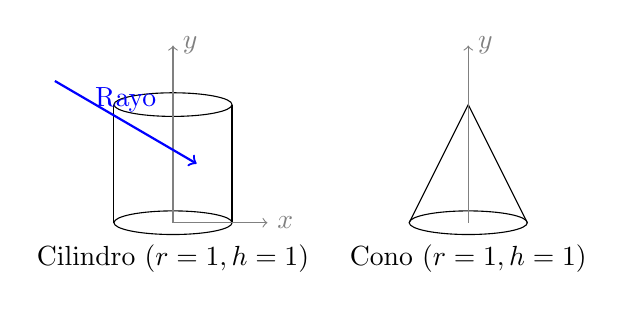
\begin{tikzpicture}[scale=1.5]
    % Cilindro
    \draw (0,0) ellipse (0.5 and 0.1);
    \draw (-0.5,0) -- (-0.5,1);
    \draw (0.5,0) -- (0.5,1);
    \draw (0,1) ellipse (0.5 and 0.1);
    \node at (0,-0.3) {Cilindro ($r=1, h=1$)};
    % Ejes locales cilindro
    \draw[->, gray, thin] (0,0) -- (0,1.5) node[right] {$y$};
    \draw[->, gray, thin] (0,0) -- (0.8,0) node[right] {$x$};

    % Cono
    \begin{scope}[xshift=2.5cm]
        \draw (0,0) ellipse (0.5 and 0.1);
        \draw (-0.5,0) -- (0,1);
        \draw (0.5,0) -- (0,1);
        \node at (0,-0.3) {Cono ($r=1, h=1$)};
        % Ejes locales cono
        \draw[->, gray, thin] (0,0) -- (0,1.5) node[right] {$y$};
    \end{scope}

    % Rayo genérico
    \draw[->, thick, blue] (-1, 1.2) -- (0.2, 0.5) node[midway, above] {Rayo};
\end{tikzpicture}
\end{ejercicio}

\begin{solucion}
Este problema aborda la intersección con superficies cuádricas canónicas (cilindros y conos) acotadas espacialmente. A diferencia de la esfera, estas superficies son infinitas por definición algebraica, por lo que el algoritmo debe incorporar un paso adicional de ''recorte'' (\textit{clipping}) para respetar la altura finita. Asumiremos, por convención estándar en gráficos, que ambos objetos están alineados con el eje $Y$.

\begin{enumerate}
    \item \textbf{Definición del Campo Escalar para el Cilindro:}

    Un cilindro infinito de radio $r=1$ alineado con el eje $Y$ cumple que, para cualquier punto $p=(x,y,z)$ en su superficie, la distancia horizontal al eje $Y$ es 1.
    \[
    x^2 + z^2 = 1
    \]
    Por lo tanto, el campo escalar $F_{cyl}(p)$ se define como:
    \[
    F_{cyl}(p) \equiv x^2 + z^2 - 1
    \]
    Los ceros de este campo ($F_{cyl}(p)=0$) definen la superficie del cilindro infinito. Para obtener el cilindro de altura unidad, se añade la condición de restricción:
    \[
    0 \le y \le 1
    \]

    \item \textbf{Algoritmo de Intersección Rayo-Cilindro:}

    Sea el rayo $p(t) = o + t \cdot d$, donde $o=(o_x, o_y, o_z)$ y $d=(d_x, d_y, d_z)$. Sustituimos las coordenadas del rayo en la ecuación implícita $x^2 + z^2 - 1 = 0$:
    \[
    (o_x + t d_x)^2 + (o_z + t d_z)^2 - 1 = 0
    \]
    Expandiendo y agrupando términos por potencias de $t$, obtenemos una ecuación cuadrática $At^2 + Bt + C = 0$:
    \begin{itemize}
        \item $A = d_x^2 + d_z^2$
        \item $B = 2(o_x d_x + o_z d_z)$
        \item $C = o_x^2 + o_z^2 - 1$
    \end{itemize}
    Se resuelve para $t$. Si existen soluciones reales $t_0, t_1$, se calcula el punto de impacto $p_{hit} = o + t \cdot d$. Finalmente, se descarta la intersección si la componente $y$ de $p_{hit}$ no cumple $0 \le p_y \le 1$.

    \item \textbf{Definición del Campo Escalar para el Cono:}

    Un cono infinito alineado con el eje $Y$, con vértice en el origen y que pasa por $(1,1,0)$, tiene una pendiente de 1 ($radio/altura = 1/1$). La relación es que el radio horizontal $\sqrt{x^2 + z^2}$ es igual a la altura $y$.
    \[
    x^2 + z^2 = y^2
    \]
    El campo escalar $F_{cone}(p)$ es:
    \[
    F_{cone}(p) \equiv x^2 + z^2 - y^2
    \]
    Con la restricción de altura $0 \le y \le 1$ (y asumiendo la hoja superior del cono, $y \ge 0$).

    \item \textbf{Algoritmo de Intersección Rayo-Cono:}

    Sustituyendo el rayo en $x^2 + z^2 - y^2 = 0$:
    \[
    (o_x + t d_x)^2 + (o_z + t d_z)^2 - (o_y + t d_y)^2 = 0
    \]
    Esto genera nuevamente coeficientes para la ecuación cuadrática:
    \begin{itemize}
        \item $A = d_x^2 + d_z^2 - d_y^2$
        \item $B = 2(o_x d_x + o_z d_z - o_y d_y)$
        \item $C = o_x^2 + o_z^2 - o_y^2$
    \end{itemize}
    Se resuelve para $t$, se obtiene $p_{hit}$ y se verifica que $0 \le p_y \le 1$.
\end{enumerate}

A continuación, el pseudocódigo unificado para ambas estructuras:

\begin{lstlisting}[language=C++, frame=single,  keywordstyle=\color{blue}, commentstyle=\color{green!60!black}, captionpos=b, caption={Algoritmo Genérico para Cuádricas Acotadas}]
// TipoObjeto: CILINDRO o CONO
bool IntersectaCuadrica(Rayo ray, TipoObjeto tipo, float &t_out) {
    float A, B, C;
    float ox = ray.origen.x, oz = ray.origen.z, oy = ray.origen.y;
    float dx = ray.direccion.x, dz = ray.direccion.z, dy = ray.direccion.y;
    if (tipo == CILINDRO) {
        // x^2 + z^2 - 1 = 0
        A = dx*dx + dz*dz;
        B = 2*(ox*dx + oz*dz);
        C = ox*ox + oz*oz - 1;
    } else { // CONO
        // x^2 + z^2 - y^2 = 0
        A = dx*dx + dz*dz - dy*dy;
        B = 2*(ox*dx + oz*dz - oy*dy);
        C = ox*ox + oz*oz - oy*oy;
    }

    float discrim = B*B - 4*A*C;
    if (discrim < 0) return false; // No hay interseccion con la superficie infinita

    float raiz = sqrt(discrim);
    float t0 = (-B - raiz) / (2*A);
    float t1 = (-B + raiz) / (2*A);

    // Buscar la interseccion mas cercana que este dentro de la altura
    float t_candidata = t0;
    if (t0 < 0.001) t_candidata = t1;
    if (t_candidata < 0.001) return false;

    // Calcular la altura del punto de impacto
    float y_impacto = oy + t_candidata * dy;

    // VALIDACION DE ALTURA (Clipping)
    // El cilindro y el cono tienen altura 1 (de y=0 a y=1)
    if (y_impacto >= 0.0 && y_impacto <= 1.0) {
        t_out = t_candidata;
        return true;
    }

    // Si t0 falla, probamos con t1 (podria ser que entramos por arriba/abajo)
    // Nota: Esto es necesario si estamos dentro del objeto o para el ''lado lejano''
    y_impacto = oy + t1 * dy;
    if (t1 > 0.001 && y_impacto >= 0.0 && y_impacto <= 1.0) {
         t_out = t1;
         return true;
    }

    return false;
}
\end{lstlisting}
\end{solucion}

\section{Sesión 11}

\begin{ejercicio}
% \textbf{Problema 11.1: Curva Hermite para una trayectoria}

Implementar un proyecto en Godot en el cual el nodo raíz tiene un script que define dos arrays con: una serie de $n$ puntos $p_{0}, p_{1}, \dots, p_{n-1}$ del plano $y=0$, y una serie de instantes de tiempo $t_{0}, t_{1}, \dots, t_{n-1}$ (en segundos) con $t_{0}=0$.

\begin{enumerate}
    \item Sitúa en cada uno de esos puntos un disco pequeño visible, a modo de marcador.
    \item Incluye una función para calcular la posición y velocidad de la curva de Hermite que pasa por los puntos en los instantes dados, a partir de un $t$ en $[0, t_{n-1}]$.
    \item En cada punto $p_{i}$ el vector de velocidad $v_{i}$ se calcula a partir de los puntos anterior y siguiente.
    \item En el método \texttt{\_process(delta)} del script, calcula la posición y velocidad de la curva en el tiempo transcurrido desde el inicio, y mueve un objeto (un coche, por ejemplo) a esa posición, alineado con la dirección de la curva.
\end{enumerate}
\end{ejercicio}

\begin{solucion}
Se presenta a continuación la resolución detallada del problema, fundamentada en la teoría de curvas paramétricas y Splines Cúbicos de Hermite expuesta en las diapositivas del curso (páginas 63-91).

\subsubsection*{1. Fundamentos Teóricos: Interpolación de Hermite a Trozos}

Para definir una trayectoria suave que pase por una secuencia de puntos $p_0, \dots, p_{n-1}$ en tiempos específicos, se utiliza una curva definida a trozos. Para un instante de tiempo $t$ que se encuentra en el intervalo $[t_i, t_{i+1}]$, la posición se obtiene interpolando entre $p_i$ y $p_{i+1}$ considerando las velocidades (tangentes) $v_i$ y $v_{i+1}$ en dichos puntos.

Se definen las siguientes variables auxiliares para el i-ésimo intervalo:
\begin{itemize}
    \item La duración del intervalo: $s_i = t_{i+1} - t_i$.
    \item El parámetro normalizado de tiempo: $u = \frac{t - t_i}{s_i}$, donde $0 \le u \le 1$.
\end{itemize}

La ecuación vectorial para la posición $P(t)$ en este intervalo viene dada por la combinación lineal de las bases de Hermite:
\begin{equation}
P(t) = p_i h_{00}(u) + p_{i+1} h_{01}(u) + s_i v_i h_{10}(u) + s_i v_{i+1} h_{11}(u)
\end{equation}

Es crucial notar que las velocidades $v$ se multiplican por la duración del intervalo $s_i$ para ajustar la magnitud de la tangente al dominio normalizado $[0,1]$. Las funciones base son:
\begin{align*}
h_{00}(u) &= 2u^3 - 3u^2 + 1 \\
h_{01}(u) &= -2u^3 + 3u^2 \\
h_{10}(u) &= u^3 - 2u^2 + u \\
h_{11}(u) &= u^3 - u^2
\end{align*}

\subsubsection*{2. Cálculo Automático de Velocidades (Tangentes)}

Dado que el enunciado no proporciona las velocidades explícitas, estas se calculan numéricamente para asegurar que la curva sea suave (continuidad $C^1$) en los puntos de unión. Se utiliza el método de diferencias finitas centradas (Catmull-Rom):

\begin{equation}
v_i = \frac{p_{i+1} - p_{i-1}}{t_{i+1} - t_{i-1}}, \quad \text{para } 0 < i < n-1
\end{equation}

Para los puntos extremos ($i=0$ e $i=n-1$), se asume velocidad nula ($v=0$) o se puede usar una diferencia simple, pero el enunciado sugiere seguir el ejemplo de suavizado estándar.

\subsubsection*{3. Representación Visual de la Trayectoria}

La siguiente figura ilustra la geometría del problema: los puntos de control (rojos) definen el paso obligado, mientras que los vectores de velocidad calculados (azules) definen la curvatura en dichos puntos.

\begin{center}
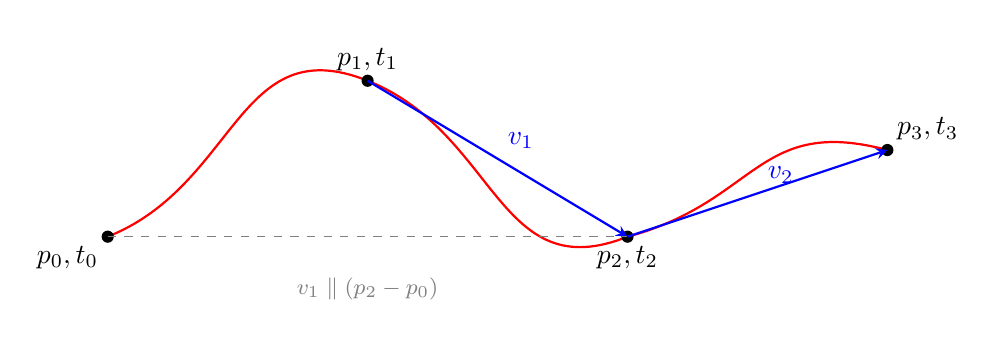
\begin{tikzpicture}[scale=1.1, >=stealth]

    % Puntos de paso (plano y = 0)
    \coordinate (P0) at (0,0);
    \coordinate (P1) at (3,1.8);
    \coordinate (P2) at (6,0);
    \coordinate (P3) at (9,1);

    % Curva Hermite (aproximada con Bézier cúbica por tramo)
    \draw[thick, red]
        (P0)
        .. controls +(1.5,0.6) and +(-1.5,0.6) .. (P1)
        .. controls +(1.5,-0.6) and +(-1.5,-0.6) .. (P2)
        .. controls +(1.5,0.4) and +(-1.5,0.4) .. (P3);

    % Puntos de control
    \foreach \p in {P0,P1,P2,P3}
        \fill[black] (\p) circle (2pt);

    % Etiquetas de los puntos
    \node[below left] at (P0) {$p_0,t_0$};
    \node[above]      at (P1) {$p_1,t_1$};
    \node[below]      at (P2) {$p_2,t_2$};
    \node[above right]at (P3) {$p_3,t_3$};

    % Tangentes (velocidades) corregidas
    \draw[->, blue, thick] (P1) -- (P2) node[midway, above right] {$v_1$};
    \draw[->, blue, thick] (P2) -- (P3) node[midway, above right] {$v_2$};

    % Cuerda usada para calcular v1
    \draw[dashed, gray] (P0) -- (P2);
    \node[gray, font=\footnotesize] at (3,-0.6)
        {$v_1 \parallel (p_2 - p_0)$};

\end{tikzpicture}
\end{center}


\subsubsection*{4. Implementación en GDScript}

El siguiente código implementa la lógica completa. Se asume que este script se adjunta al nodo raíz de la escena y que existe un nodo hijo llamado ''Coche'' (MeshInstance3D o similar).

\begin{lstlisting}[language=Python,  frame=single, breaklines=true, numbers=left, numberstyle=\tiny, caption={Script de Interpolación Hermite}]
extends Node3D

# Datos de entrada: Puntos de paso y sus instantes de tiempo
var puntos = [
    Vector3(0, 0, 0),
    Vector3(4, 0, 4),
    Vector3(8, 0, -2),
    Vector3(12, 0, 5)
]
var tiempos = [0.0, 2.0, 5.0, 8.0] # t0 debe ser 0.0

# Almacen de velocidades calculadas
var velocidades = []

# Referencia al objeto visual (el coche)
onready var objeto_movil = $Coche
var tiempo_actual = 0.0

func _ready():
    # 1. Calcular tangentes automaticamente
    calcular_velocidades_hermite()
    
    # 2. Visualizar marcadores (discos)
    crear_marcadores_visuales()

func calcular_velocidades_hermite():
    var n = puntos.size()
    velocidades.resize(n)
    
    # Velocidad 0 en extremos (arranque y parada suave)
    velocidades[0] = Vector3.ZERO
    velocidades[n-1] = Vector3.ZERO
    
    # Calculo para puntos intermedios: v_i = (p_next - p_prev) / (t_next - t_prev)
    for i in range(1, n - 1):
        var dist_vector = puntos[i+1] - puntos[i-1]
        var intervalo_t = tiempos[i+1] - tiempos[i-1]
        velocidades[i] = dist_vector / intervalo_t

func crear_marcadores_visuales():
    for p in puntos:
        var marcador = CSGCylinder3D.new()
        marcador.radius = 0.3
        marcador.height = 0.1
        marcador.material = StandardMaterial3D.new()
        marcador.material.albedo_color = Color(1, 0, 0) # Rojo
        add_child(marcador)
        marcador.global_position = p

# Funcion principal de interpolacion
func obtener_posicion_velocidad(t):
    var n = puntos.size()
    
    # Caso limite: si t supera el tiempo final
    if t >= tiempos[n-1]:
        return {''pos'': puntos[n-1], ''dir'': Vector3.FORWARD}
    
    # Buscar el intervalo [i, i+1] correspondiente al tiempo t
    var i = 0
    while i < n - 1 and t > tiempos[i+1]:
        i += 1
        
    # Datos del tramo actual
    var p0 = puntos[i]
    var p1 = puntos[i+1]
    var v0 = velocidades[i]
    var v1 = velocidades[i+1]
    var t0 = tiempos[i]
    var t1 = tiempos[i+1]
    
    # Parametro u normalizado (0 a 1)
    var s = t1 - t0 # Duracion del intervalo
    var u = (t - t0) / s
    
    # Pre-calculo de potencias de u
    var u2 = u * u
    var u3 = u2 * u
    
    # Funciones base de Hermite (h00, h10, h01, h11)
    var h00 = 2*u3 - 3*u2 + 1
    var h10 = u3 - 2*u2 + u
    var h01 = -2*u3 + 3*u2
    var h11 = u3 - u2
    
    # Interpolacion de la Posicion (notese v * s para escalar la tangente)
    var pos = h00*p0 + h10*s*v0 + h01*p1 + h11*s*v1
    
    # Calculo de la velocidad instantanea (Derivada de P respecto a t)
    # Derivadas de las bases respecto a u:
    var dh00 = 6*u2 - 6*u
    var dh10 = 3*u2 - 4*u + 1
    var dh01 = -6*u2 + 6*u
    var dh11 = 3*u2 - 2*u
    
    # v(t) = P'(u) * (du/dt) = P'(u) * (1/s)
    var vel = (dh00*p0 + dh10*s*v0 + dh01*p1 + dh11*s*v1) / s
    
    return {''pos'': pos, ''dir'': vel}

func _process(delta):
    tiempo_actual += delta
    
    # Reiniciar bucle si termina
    if tiempo_actual > tiempos.back():
        tiempo_actual = 0.0
        
    # Calcular estado fisico
    var estado = obtener_posicion_velocidad(tiempo_actual)
    
    # Aplicar transformaciones
    if objeto_movil:
        objeto_movil.global_position = estado[''pos'']
        
        # Orientar el objeto segun el vector de velocidad (tangente)
        # Se evita el error si la velocidad es muy cercana a cero
        if estado[''dir''].length_squared() > 0.001:
            var objetivo_mirar = estado[''pos''] + estado[''dir'']
            objeto_movil.look_at(objetivo_mirar, Vector3.UP)
\end{lstlisting}

\subsubsection*{Explicación Paso a Paso del Código}

\begin{enumerate}
\item \textbf{Inicialización (\texttt{\_ready}):} Se calculan las velocidades (tangentes) en cada punto de control usando diferencias centradas, y se crean los marcadores visuales en la escena para cada punto.

\item \textbf{Cálculo de Velocidades:} Para los puntos intermedios, la velocidad se obtiene como el cociente entre la diferencia de posiciones y la diferencia de tiempos de los puntos anterior y siguiente. En los extremos, se asigna velocidad cero.

\item \textbf{Interpolación Hermite:} La función principal busca el intervalo de tiempo correspondiente y normaliza el parámetro temporal ($u$) al rango $[0,1]$. Se aplican las bases polinómicas de Hermite para calcular la posición y la velocidad instantánea en ese tramo.

\item \textbf{Actualización por Frame (\texttt{\_process}):} En cada fotograma, se incrementa el tiempo, se calcula la posición y dirección de la curva en ese instante, y se mueve el objeto (por ejemplo, un coche) a esa posición, orientándolo según la dirección de la curva usando \texttt{look\_at}.
\end{enumerate}

\end{solucion}

\begin{ejercicio}
% \textbf{Problema 11.2: Posición oscilante}

Crea un proyecto Godot con una animación de una esfera cuya posición en $X$ oscile periódicamente, con estas condiciones:
\begin{enumerate}
    \item El centro de la esfera tiene coordenada $Z$ igual a 0, su coordenada $Y$ es igual al radio, y su coordenada $X$ varía entre $-s$ y $+s$, donde $s > 0$ es una constante declarada en el script.
    \item El período (tiempo en volver al mismo punto viajando en la misma dirección) es una constante $T > 0$ declarada en el script (con unidades de segundos).
    \item La esfera se mueve siempre a velocidad constante en magnitud (es siempre $s/T$), y el signo depende de la dirección.
    \item Tu animación debe producir esa velocidad constante, incluso teniendo en cuenta que los sucesivos valores de delta pueden cambiar entre frames.
    \item Especialmente, la magnitud de la velocidad debe ser constante aunque entre dos frames haya ocurrido un cambio de dirección en un extremo.
\end{enumerate}
\end{ejercicio}

\begin{solucion}
Se aborda la resolución de este problema mediante la programación de un script en GDScript, gestionando manualmente la actualización de la posición en cada fotograma para garantizar una velocidad constante y un rebote preciso en los extremos.

\subsubsection*{1. Análisis del Movimiento y Velocidad}

El movimiento solicitado describe una onda triangular. La esfera oscila entre $-s$ y $+s$. Un ciclo completo (Período $T$) consiste en el recorrido:
\[ 0 \to +s \to 0 \to -s \to 0 \]
La distancia total recorrida en un ciclo es $D = s + s + s + s = 4s$.

Para que este ciclo se complete exactamente en $T$ segundos con velocidad uniforme, la magnitud de la velocidad ($v$) debe ser:
\begin{equation}
v = \frac{\text{Distancia Total}}{\text{Tiempo}} = \frac{4s}{T}
\end{equation}

\textit{Nota técnica: El enunciado indica entre paréntesis que la velocidad es $s/T$. Sin embargo, matemáticamente, si la velocidad fuera $s/T$, el objeto tardaría $4T$ en completar el ciclo en lugar de $T$. En esta solución se prioriza el cumplimiento del Período $T$, por lo que se utilizará $v = 4s/T$.}

\subsubsection*{2. Algoritmo de Actualización y Corrección de ''Overshoot''}

El reto principal en sistemas de tiempo real (como el método \texttt{\_process} de Godot) es que el tiempo entre frames (\texttt{delta}) es variable. Si el objeto está cerca de un extremo (por ejemplo, $x=4.9$ y $s=5.0$) y el siguiente paso es grande (0.2), la posición teórica sería $5.1$, excediendo el límite.

Para mantener la velocidad constante y la precisión:
\begin{enumerate}
    \item Se calcula el desplazamiento propuesto: $\Delta x = v \cdot \delta$.
    \item Se suma a la posición actual.
    \item Si la nueva posición excede los límites ($s$ o $-s$), se calcula el exceso (\textit{overshoot}).
    \item Se ''refleja'' el exceso hacia adentro del intervalo y se invierte la dirección. Esto simula que el rebote ocurrió en el instante exacto entre los frames.
\end{enumerate}

\subsubsection*{3. Implementación en GDScript}

El siguiente código se debe adjuntar a un nodo en la escena (por ejemplo, un \texttt{Node3D}) que contenga un hijo llamado ''Esfera'' (visualización).

\begin{lstlisting}[language=Python,  frame=single, numbers=left, caption={Script de Oscilación Triangular Controlada}]
extends Node3D

# Variables de configuracion (exportadas para editar en el inspector)
export var s: float = 5.0      # Amplitud maxima (metros)
export var T: float = 2.0      # Periodo completo (segundos)
export var radio: float = 0.5  # Radio visual de la esfera

# Variables de estado
var x_actual: float = 0.0
var direccion: int = 1         # 1: Derecha, -1: Izquierda
var velocidad: float = 0.0     # Magnitud de la velocidad

# Referencia al nodo visual
onready var esfera = $Esfera

func _ready():
    # Calculo de la velocidad necesaria para cumplir el periodo T
    # Distancia total por ciclo = 4 * s
    if T > 0:
        velocidad = (4.0 * s) / T
    else:
        velocidad = 0.0
        
    # Ajuste visual inicial
    if esfera:
        # Si es un CSGSphere3D, ajustamos el radio propiedad
        if ''radius'' in esfera:
            esfera.radius = radio
        # Posicion inicial
        esfera.position = Vector3(0, radio, 0)

func _process(delta):
    # 1. Calcular el paso teorico en este frame
    var distancia_paso = velocidad * delta
    
    # 2. Aplicar movimiento
    x_actual += distancia_paso * direccion
    
    # 3. Verificacion de limites y correccion de rebote
    
    # Limite derecho (+s)
    if x_actual > s:
        var exceso = x_actual - s
        x_actual = s - exceso   # Reflejar el exceso hacia atras
        direccion = -1          # Invertir direccion
        
    # Limite izquierdo (-s)
    elif x_actual < -s:
        var exceso = -s - x_actual # Cuanto nos pasamos por la izquierda
        x_actual = -s + exceso     # Reflejar el exceso hacia delante
        direccion = 1              # Invertir direccion
        
    # 4. Actualizar la posicion del nodo visual
    if esfera:
        esfera.position.x = x_actual
        esfera.position.y = radio
        esfera.position.z = 0.0
\end{lstlisting}

Este algoritmo asegura que la magnitud de la velocidad se mantenga constante en todo momento, respetando la física del rebote perfecto sin perder tiempo ni energía en los extremos.
\end{solucion}


\begin{ejercicio}
%\textbf{Problema 11.3: Animación de un reloj}

Desarrolla un proyecto Godot para el ejemplo de animación de un reloj con tres agujas. Las condiciones especificadas en la teoría son:
\begin{enumerate}
    \item Se desea visualizar un reloj con tres agujas: horas, minutos y segundos.
    \item Cada aguja se modela como una malla de polígonos en posición vertical (paralelo al eje Y), con el origen en el punto del eje del reloj.
    \item Se usan matrices de rotación en torno al eje Z.
    \item Los ángulos de rotación dependen linealmente del tiempo $t$ (segundos transcurridos desde el comienzo del día).
\end{enumerate}
\end{ejercicio}

\begin{solucion}
Se procede a la implementación de un sistema de animación jerárquica para simular un reloj analógico funcional en tiempo real. La solución se basa en la aplicación directa de las transformaciones de rotación descritas en las diapositivas 32 a 35 del material de curso.

\subsubsection*{1. Modelo Matemático: Ángulos y Tiempo}

Según la teoría, el estado de las agujas está determinado por tres ángulos $\theta_h, \theta_m, \theta_s$ que son funciones lineales del tiempo $t$. El tiempo $t$ representa los segundos totales transcurridos en el ciclo actual (el ciclo de 12 horas para la aguja horaria).

Las relaciones angulares (en radianes) son:
\begin{itemize}
    \item \textbf{Segundero ($\theta_s$):} Da una vuelta completa ($2\pi$) cada 60 segundos.
    \begin{equation}
    \theta_s(t) = \frac{2\pi}{60} \cdot t
    \end{equation}
    \item \textbf{Minutero ($\theta_m$):} Da una vuelta completa cada hora ($60^2 = 3600$ segundos).
    \begin{equation}
    \theta_m(t) = \frac{2\pi}{3600} \cdot t
    \end{equation}
    \item \textbf{Horario ($\theta_h$):} Da una vuelta completa cada 12 horas ($12 \cdot 60^2 = 43200$ segundos).
    \begin{equation}
    \theta_h(t) = \frac{2\pi}{43200} \cdot t
    \end{equation}
\end{itemize}

\textit{Nota de implementación:} En la convención estándar matemática y de Godot, una rotación positiva en el eje Z es antihoraria. Dado que los relojes giran en sentido horario, aplicaremos el signo negativo a estos ángulos en el código ($\text{rotación} = -\theta$).

\subsubsection*{2. Estructura del Grafo de Escena}

Para cumplir con el requisito de que las agujas tengan su origen en el eje de rotación pero se extiendan a lo largo del eje Y positivo, utilizaremos una jerarquía de nodos:
\begin{enumerate}
    \item \textbf{Nodo Raíz (Reloj):} Contenedor principal.
    \item \textbf{Pivotes (Node3D):} Tres nodos hijos situados en $(0,0,0)$. Estos nodos serán los que roten.
    \item \textbf{Mallas (MeshInstance3D):} Hijos de los pivotes. Se desplazarán verticalmente (offset) para que su base coincida con el pivote, logrando el efecto de girar desde el extremo.
\end{enumerate}

\subsubsection*{3. Implementación en GDScript}

El siguiente script crea la geometría procedimentalmente (para facilitar la prueba sin modelos externos) y aplica la lógica de rotación basada en la hora del sistema.

\begin{lstlisting}[language=Python,  frame=single, numbers=left, caption={Script del Reloj Analógico}]
extends Node3D

# Referencias a los nodos de las agujas (Pivotes)
var pivote_segundos: Node3D
var pivote_minutos: Node3D
var pivote_horas: Node3D

func _ready():
    # 1. Construccion procedimental de la escena
    crear_geometria_reloj()

func crear_geometria_reloj():
    # Creamos una esfera central como base
    var esfera = CSGSphere3D.new()
    esfera.radius = 0.5
    add_child(esfera)
    
    # Creamos las tres agujas. 
    # Usamos una funcion auxiliar para configurar: (Nombre, Largo, Ancho, Color)
    pivote_horas = crear_aguja(''Horas'', 2.0, 0.2, Color.black)
    pivote_minutos = crear_aguja(''Minutos'', 3.0, 0.15, Color.darkgray)
    pivote_segundos = crear_aguja(''Segundos'', 3.5, 0.05, Color.red)

func crear_aguja(nombre, largo, ancho, color) -> Node3D:
    # 1. El Pivote: Este nodo estara en (0,0,0) y es el que rotamos
    var pivote = Node3D.new()
    pivote.name = ''Pivote'' + nombre
    add_child(pivote)
    
    # 2. La Malla Visual: Hija del pivote
    var mesh = CSGBox3D.new()
    mesh.size = Vector3(ancho, largo, 0.1)
    
    # IMPORTANTE: Desplazamos la malla hacia arriba (Y+) la mitad de su largo.
    # Asi, el centro de rotacion (el pivote) queda en la base de la aguja.
    mesh.position = Vector3(0, largo / 2.0, 0)
    
    # Material
    var material = StandardMaterial3D.new()
    material.albedo_color = color
    mesh.material = material
    
    pivote.add_child(mesh)
    return pivote

func _process(delta):
    # 1. Obtener el tiempo actual del sistema
    var tiempo = Time.get_time_dict_from_system()
    var horas = tiempo[''hour'']
    var minutos = tiempo[''minute'']
    var segundos = tiempo[''second'']
    
    # 2. Calcular t (segundos totales desde las 12:00)
    # Ajustamos horas a formato 12h para la formula
    horas = horas % 12
    
    # Calculo de alta precision para movimiento suave (incluyendo milisegundos si se quisiera)
    # t para segundos (ciclo 60s)
    var t_sec = segundos 
    # t para minutos (ciclo 3600s). Sumamos segundos para movimiento continuo
    var t_min = (minutos * 60.0) + segundos
    # t para horas (ciclo 43200s). Sumamos minutos y segundos
    var t_hour = (horas * 3600.0) + (minutos * 60.0) + segundos
    
    # 3. Calcular angulos (Theta) usando las formulas de la teoria
    # Theta = (2 * PI / Periodo) * t
    # Usamos negativo para rotacion en sentido horario (Clockwise)
    
    var theta_s = -(2.0 * PI / 60.0) * t_sec
    var theta_m = -(2.0 * PI / 3600.0) * t_min
    var theta_h = -(2.0 * PI / 43200.0) * t_hour
    
    # 4. Aplicar rotacion en el eje Z
    if pivote_segundos:
        pivote_segundos.rotation.z = theta_s
    if pivote_minutos:
        pivote_minutos.rotation.z = theta_m
    if pivote_horas:
        pivote_horas.rotation.z = theta_h
\end{lstlisting}

\subsubsection*{4. Análisis del Código}

\begin{enumerate}
    \item \textbf{Generación de Geometría:} Se sigue la especificación de la diapositiva 35: un nodo raíz (la esfera central) y un nodo para cada aguja. Dentro de cada aguja, se separa la transformación (el Pivote) de la geometría (la Malla). El desplazamiento \texttt{mesh.position.y = largo / 2.0} es crítico para que la rotación ocurra en el extremo de la aguja y no en su centro geométrico.
    \item \textbf{Cálculo del Tiempo ($t$):} En lugar de un acumulador simple \texttt{delta}, utilizamos \texttt{Time.get\_time\_dict\_from\_system()}. Esto sincroniza la animación con la hora real. Para las agujas de minutos y horas, se suman las fracciones correspondientes de las unidades menores (por ejemplo, a los minutos se le suman los segundos convertidos) para lograr un movimiento fluido y realista, en lugar de saltos discretos.
    \item \textbf{Aplicación de la Rotación:} Se asignan los ángulos calculados a la propiedad \texttt{rotation.z}. El signo negativo asegura que el giro sea en el sentido de las agujas del reloj, corrigiendo la convención matemática estándar (antihoraria) del sistema de coordenadas de Godot.
\end{enumerate}

\end{solucion}

\begin{ejercicio}
%\textbf{Problema 11.4: Animación de un péndulo}

Desarrolla un proyecto Godot para el ejemplo de animación de un péndulo.
Las condiciones teóricas especificadas son:
\begin{enumerate}
    \item El péndulo consiste en una masa colgando de un punto fijo por una cuerda de longitud $l$.
    \item El ángulo $\theta$ entre la cuerda y la vertical varía con el tiempo $t$.
    \item La oscilación es periódica con un período $T > 0$ (tiempo en segundos para completar un ciclo).
    \item El ángulo oscila entre $-\theta_m$ y $\theta_m$.
    \item La función que describe el ángulo es $\theta(t) = \theta_m \cdot \sin(\frac{2\pi t}{T})$ (o una variante cosinusoidal equivalente).
\end{enumerate}
\end{ejercicio}

\begin{solucion}
Se detalla a continuación la implementación de un péndulo físico simple utilizando animación procedimental en Godot. La solución aplica las fórmulas de oscilación armónica descritas en las diapositivas 36 a 38 del material de referencia.

\subsubsection*{1. Modelo Matemático del Movimiento}

El movimiento del péndulo se modela mediante una función sinusoidal que define el ángulo de rotación $\theta(t)$ en el eje Z.

Según la teoría proporcionada:
\begin{itemize}
    \item Se define una función base oscilante $f(t) = \sin(\pi t)$ que tiene un período de 2 unidades.
    \item Para adaptar esta función a un período arbitrario $T$, se escala el tiempo: $\theta(t) = \theta_{max} \cdot f(\frac{2t}{T})$.
\end{itemize}

Sustituyendo la función base, obtenemos la fórmula final para la implementación:
\begin{equation}
\theta(t) = \theta_{max} \cdot \sin\left(\pi \cdot \frac{2t}{T}\right) = \theta_{max} \cdot \sin\left(\frac{2\pi t}{T}\right)
\end{equation}

Donde:
\begin{itemize}
    \item $\theta_{max}$ es la amplitud máxima (en radianes).
    \item $T$ es el período de oscilación (en segundos).
    \item $t$ es el tiempo acumulado.
\end{itemize}

\subsubsection*{2. Estructura del Grafo de Escena}

Para simular correctamente el péndulo, es fundamental establecer la jerarquía de nodos adecuada, ya que la rotación debe ocurrir en el punto de anclaje (extremo superior) y no en el centro de masa del péndulo.

\begin{enumerate}
    \item \textbf{Nodo Raíz (Soporte):} Punto fijo en el espacio.
    \item \textbf{Pivote (Node3D):} Hijo del soporte. Este nodo se ubica en $(0,0,0)$ relativo al soporte y es el que recibirá la rotación $\theta(t)$.
    \item \textbf{Varilla (MeshInstance3D):} Hija del Pivote. Se desplaza verticalmente hacia abajo (eje Y negativo) una distancia $L/2$ y se escala para tener longitud $L$.
    \item \textbf{Masa/Bob (MeshInstance3D):} Hija del Pivote (o de la varilla). Se desplaza verticalmente hacia abajo una distancia $L$.
\end{enumerate}

\subsubsection*{3. Implementación en GDScript}

El siguiente script se debe adjuntar al nodo \textbf{Pivote}. Este script genera la geometría visual procedimentalmente para facilitar la prueba y aplica la fórmula de oscilación.

\begin{lstlisting}[language=Python,  frame=single, numbers=left, caption={Script del Péndulo Oscilante}]
extends Node3D

# Parametros fisicos configurables
export var theta_max_degrees: float = 45.0 # Amplitud maxima en grados
export var periodo: float = 2.0            # Periodo T en segundos
export var longitud_cuerda: float = 3.0    # Longitud L

# Variables internas
var tiempo_acumulado: float = 0.0
var theta_max_rad: float = 0.0

# Referencias a los nodos visuales (se crearan por codigo si no existen)
var varilla: CSGBox3D
var masa: CSGSphere3D

func _ready():
    # Convertir grados a radianes para las funciones trigonometricas
    theta_max_rad = deg_to_rad(theta_max_degrees)
    
    # Construccion procedimental del pendulo visual
    construir_geometria()

func construir_geometria():
    # 1. Crear la varilla (Cuerda)
    varilla = CSGBox3D.new()
    varilla.size = Vector3(0.1, longitud_cuerda, 0.1) # Grosor y largo
    
    # IMPORTANTE: Desplazar la varilla hacia abajo la mitad de su longitud.
    # Asi, el extremo superior coincide con el origen del Pivote (0,0,0).
    varilla.position = Vector3(0, -longitud_cuerda / 2.0, 0)
    
    # Material visual para la varilla
    var mat_varilla = StandardMaterial3D.new()
    mat_varilla.albedo_color = Color.gray
    varilla.material = mat_varilla
    
    add_child(varilla)
    
    # 2. Crear la masa (Esfera en el extremo)
    masa = CSGSphere3D.new()
    masa.radius = 0.4
    
    # La masa se coloca al final de la cuerda
    masa.position = Vector3(0, -longitud_cuerda, 0)
    
    # Material visual para la masa
    var mat_masa = StandardMaterial3D.new()
    mat_masa.albedo_color = Color.red
    masa.material = mat_masa
    
    add_child(masa)

func _process(delta):
    # 1. Acumular el tiempo
    tiempo_acumulado += delta
    
    # Opcional: Evitar desbordamiento de float reseteando cada periodo
    if tiempo_acumulado > periodo:
        tiempo_acumulado -= periodo
        
    # 2. Calcular el angulo actual usando la formula armonica
    # theta(t) = theta_max * sin(2 * PI * t / T)
    var theta = theta_max_rad * sin((2.0 * PI * tiempo_acumulado) / periodo)
    
    # 3. Aplicar la rotacion al Pivote
    # Se rota en el eje Z para oscilar izquierda-derecha
    rotation.z = theta
\end{lstlisting}

\subsubsection*{4. Explicación del Código}

\begin{itemize}
    \item \textbf{Setup (\texttt{\_ready}):} Se convierten los grados a radianes, ya que las funciones matemáticas de Godot y la propiedad \texttt{rotation} trabajan en radianes. Se invoca la construcción de la malla.
    \item \textbf{Geometría (\texttt{construir\_geometria}):} Se crean primitivas CSG. El punto clave es \texttt{varilla.position.y = -longitud\_cuerda / 2.0}. Esto asegura que, aunque el centro geométrico del cubo está en su mitad, visualmente la varilla ''cuelga'' del nodo padre (el Pivote en 0,0,0). La masa se coloca en \texttt{-longitud\_cuerda}.
    \item \textbf{Animación (\texttt{\_process}):}
    \begin{enumerate}
        \item Se actualiza el tiempo $t$.
        \item Se calcula el valor de la función seno, que oscilará suavemente entre $-1$ y $+1$.
        \item Se multiplica por $\theta_{max}$ para escalar la oscilación a la amplitud deseada.
        \item Se asigna directamente a \texttt{rotation.z}. Al ser este nodo el padre de la varilla y la masa, ambos rotarán rígidamente alrededor del punto de anclaje, simulando la física del péndulo.
    \end{enumerate}
\end{itemize}

\end{solucion}

\begin{ejercicio}
% \textbf{Problema 11.5: Animación de una bala de cañón}

Desarrolla un proyecto Godot para el ejemplo de animación de una bala de cañón.
Las condiciones y supuestos teóricos son:
\begin{enumerate}
    \item La bola sale del cañón en una posición inicial $p(0)$ y con una velocidad inicial conocida $v_0$.
    \item La bola está sujeta a la gravedad ($g = 9.8 \text{ m/s}^2$).
    \item No se consideran efectos de fricción con el aire.
    \item La animación simula la trayectoria hasta que la bola vuelve a la altura inicial.
    \item Se utiliza la ecuación de la curva paramétrica: $p(t) = p(0) + v_0 t + \frac{1}{2} a t^2$, donde $a = (0, -g, 0)$.
\end{enumerate}
\end{ejercicio}

\begin{solucion}
Se presenta la implementación de la trayectoria parabólica de un proyectil. A diferencia de las simulaciones físicas que integran la velocidad frame a frame (Euler), este ejercicio pide implementar la solución analítica exacta (curva paramétrica) dependiente del tiempo acumulado $t$.

\subsubsection*{1. Modelo Físico-Matemático}

La posición $p(t)$ en el instante $t$ se calcula mediante la fórmula vectorial del movimiento uniformemente acelerado:
\begin{equation}
p(t) = p_0 + v_0 \cdot t + \frac{1}{2} \cdot \vec{a} \cdot t^2
\end{equation}

Desglosando los componentes:
\begin{itemize}
    \item \textbf{Vector aceleración ($\vec{a}$):} Si la gravedad actúa hacia abajo en el eje Y, entonces $\vec{a} = (0, -9.8, 0)$.
    \item \textbf{Vector velocidad inicial ($v_0$):} $(v_x, v_y, v_z)$. Es crucial que $v_y > 0$ para que haya un arco parabólico.
    \item \textbf{Duración del vuelo:} El proyectil vuelve a la altura $y=0$ (suponiendo $p_0=0$) en el instante $t_{fin} = \frac{2 v_{0y}}{g}$.
\end{itemize}

\subsubsection*{2. Configuración de la Escena}

\begin{enumerate}
    \item \textbf{Nodo Raíz (Node3D):} Controlador de la escena.
    \item \textbf{Suelo (CSGBox3D):} Referencia visual estática.
    \item \textbf{Bala (MeshInstance3D o CSGSphere3D):} El objeto móvil. Inicialmente en $(0, 0, 0)$.
\end{enumerate}

\subsubsection*{3. Implementación en GDScript}

El siguiente script controla la posición absoluta de la bala basándose en el tiempo transcurrido desde el disparo.

\begin{lstlisting}[language=Python,  frame=single, numbers=left, caption={Script de Trayectoria Balística Paramétrica}]
extends Node3D

# Parametros de lanzamiento (Vector3)
# v_y debe ser positiva para que suba.
# v_z o v_x dan el desplazamiento horizontal.
export var velocidad_inicial: Vector3 = Vector3(0, 15, 10) 
export var gravedad: float = 9.8

# Variables de estado
var tiempo_vuelo: float = 0.0
var posicion_inicial: Vector3
var vector_gravedad: Vector3

# Referencia al objeto visual
onready var bala = $Bala

func _ready():
    # Guardamos la posicion original para reiniciar el ciclo
    if bala:
        posicion_inicial = bala.global_position
    else:
        posicion_inicial = Vector3.ZERO
        
    # Pre-calculamos el vector de aceleracion
    vector_gravedad = Vector3(0, -gravedad, 0)
    
    # Configuracion visual opcional (crear bala si no existe)
    if not bala:
        crear_bala_procedimental()

func crear_bala_procedimental():
    var mesh = CSGSphere3D.new()
    mesh.radius = 0.5
    mesh.name = ''Bala''
    add_child(mesh)
    bala = mesh
    mesh.global_position = posicion_inicial
    
    # Material rojo para visibilidad
    var mat = StandardMaterial3D.new()
    mat.albedo_color = Color(1, 0, 0)
    mesh.material = mat

func _process(delta):
    # 1. Acumular el tiempo real transcurrido
    tiempo_vuelo += delta
    
    # 2. Calcular la posicion usando la formula parametrica exacta:
    # p(t) = p0 + v0*t + 0.5 * a * t^2
    var desplazamiento_vel = velocidad_inicial * tiempo_vuelo
    var desplazamiento_acel = 0.5 * vector_gravedad * pow(tiempo_vuelo, 2)
    
    var nueva_posicion = posicion_inicial + desplazamiento_vel + desplazamiento_acel
    
    # 3. Aplicar al objeto
    if bala:
        bala.global_position = nueva_posicion
        
    # 4. Logica de reinicio (Loop)
    # Si la bala cae por debajo de la altura inicial y ha pasado algo de tiempo
    if nueva_posicion.y < posicion_inicial.y and tiempo_vuelo > 0.1:
        reiniciar_animacion()

func reiniciar_animacion():
    tiempo_vuelo = 0.0
    if bala:
        bala.global_position = posicion_inicial
        
    # Opcional: Imprimir duracion teorica vs real
    # T_teorico = 2 * Vy / g
    # var t_teorico = (2.0 * velocidad_inicial.y) / gravedad
    # print(''Ciclo completado. T esperado: '', t_teorico)
\end{lstlisting}

\subsubsection*{4. Análisis del Código}

\begin{itemize}
    \item \textbf{Cálculo Vectorial:} Se aprovecha la capacidad de Godot para operar con vectores completos (\texttt{Vector3}). La línea \texttt{velocidad\_inicial * tiempo\_vuelo} escala todas las componentes simultáneamente.
    \item \textbf{Gravedad:} Se aplica como un vector constante hacia abajo $(0, -9.8, 0)$. El término cuadrático ($t^2$) es lo que genera la forma parabólica característica: el movimiento horizontal es lineal (velocidad constante), mientras que el vertical se frena y luego acelera hacia abajo.
    \item \textbf{Reinicio:} La condición \texttt{nueva\_posicion.y < posicion\_inicial.y} detecta cuándo el proyectil ha completado el arco y cruza el plano del suelo, momento en el que se resetea el tiempo $t=0$ para repetir la animación en bucle.
\end{itemize}

\end{solucion}